\subsection{Electron Fake Rate}
This section presents in more detail the studies on the electron fake rate measurement.

\subsubsection{Fakeable Object}
We perform the fake rate measurement using a number of different electron fakeable 
object definitions defined in Sec.~\ref{sec:fakerateDenominatorObjectDef}, 
each giving different performance in terms of systematic uncertainties. 
One of the two main systematic uncertainties associated with
the fake rate method is the uncertainty on the $p_{T}$
spectrum of the jet or parton from which the fake electron originates. 
Extrapolations in isolation, such as the V1 or V3 fakeable object, is susceptible
to these uncertainties. The V2 and V4 fakeable objects are already fully or 
partially isolated and therefore yield smaller systematic uncertainties due
to the jet $p_{T}$ spectrum. These options are intended to explore
the performance differences in the trade-off between jet $p_{T}$ spectrum systematic
uncertainties and statistical uncertainties in the fake rate extrapolation.


\subsubsection{Calibration Sample Selection}
\label{sec:ElectronFakeRate_CalibrationSampleSelection}
The electron fake rate is measured two orthogonal calibration samples, intended to 
capture different fake composition. The first sample is a QCD-dominated event sample
selected by events triggered by {\bf Ele8\_CaloIdL\_CaloIsoVL } or 
{\bf Ele17\_CaloIdL\_CaloIsoVL }. We impose a few additional requirements in order
to reduce contamination due to events containing electrons from $W$ and $Z$ decays:

\begin{itemize}
  \item $Z$ veto: reject the event if there are more than one reconstructed electrons,
  \item $W$ veto: reject the event if PF-MET $> 20\:\GeV$.
\end{itemize}

In order to study the dependance of the fake rate on the $p_{T}$ of the jet from which
the fake electron originates, we impose requirements on the $p_{T}$ of the leading jet 
in the event. The jet is required to have $\Delta$ R $ > 1.0$ 
to the fake electron candidate. The jets used in this study have the L1FastJet, L2Relative, and
L3Absolute jet energy corrections applied. 

\subsubsection{Fake Rates}
The electron fake rates measured in the 2011A data requiring the leading jet $p_{T}$ to be 
larger than $30$ GeV for the different fakeable object 
definitions described above are shown in Figures \ref{fig:ele_fr_V1_jet30},
\ref{fig:ele_fr_V2_jet30}, \ref{fig:ele_fr_V3_jet30}, \ref{fig:ele_fr_V4_jet30}, as a function of the 
$p_{T}$, $\eta$, and $phi$ of the electron, comparing the result measured from data to the
results from the QCD (Pt-hat 30-50) and the W+Jet Monte Carlo simulation.

\begin{figure}[!htbp]
\begin{center}
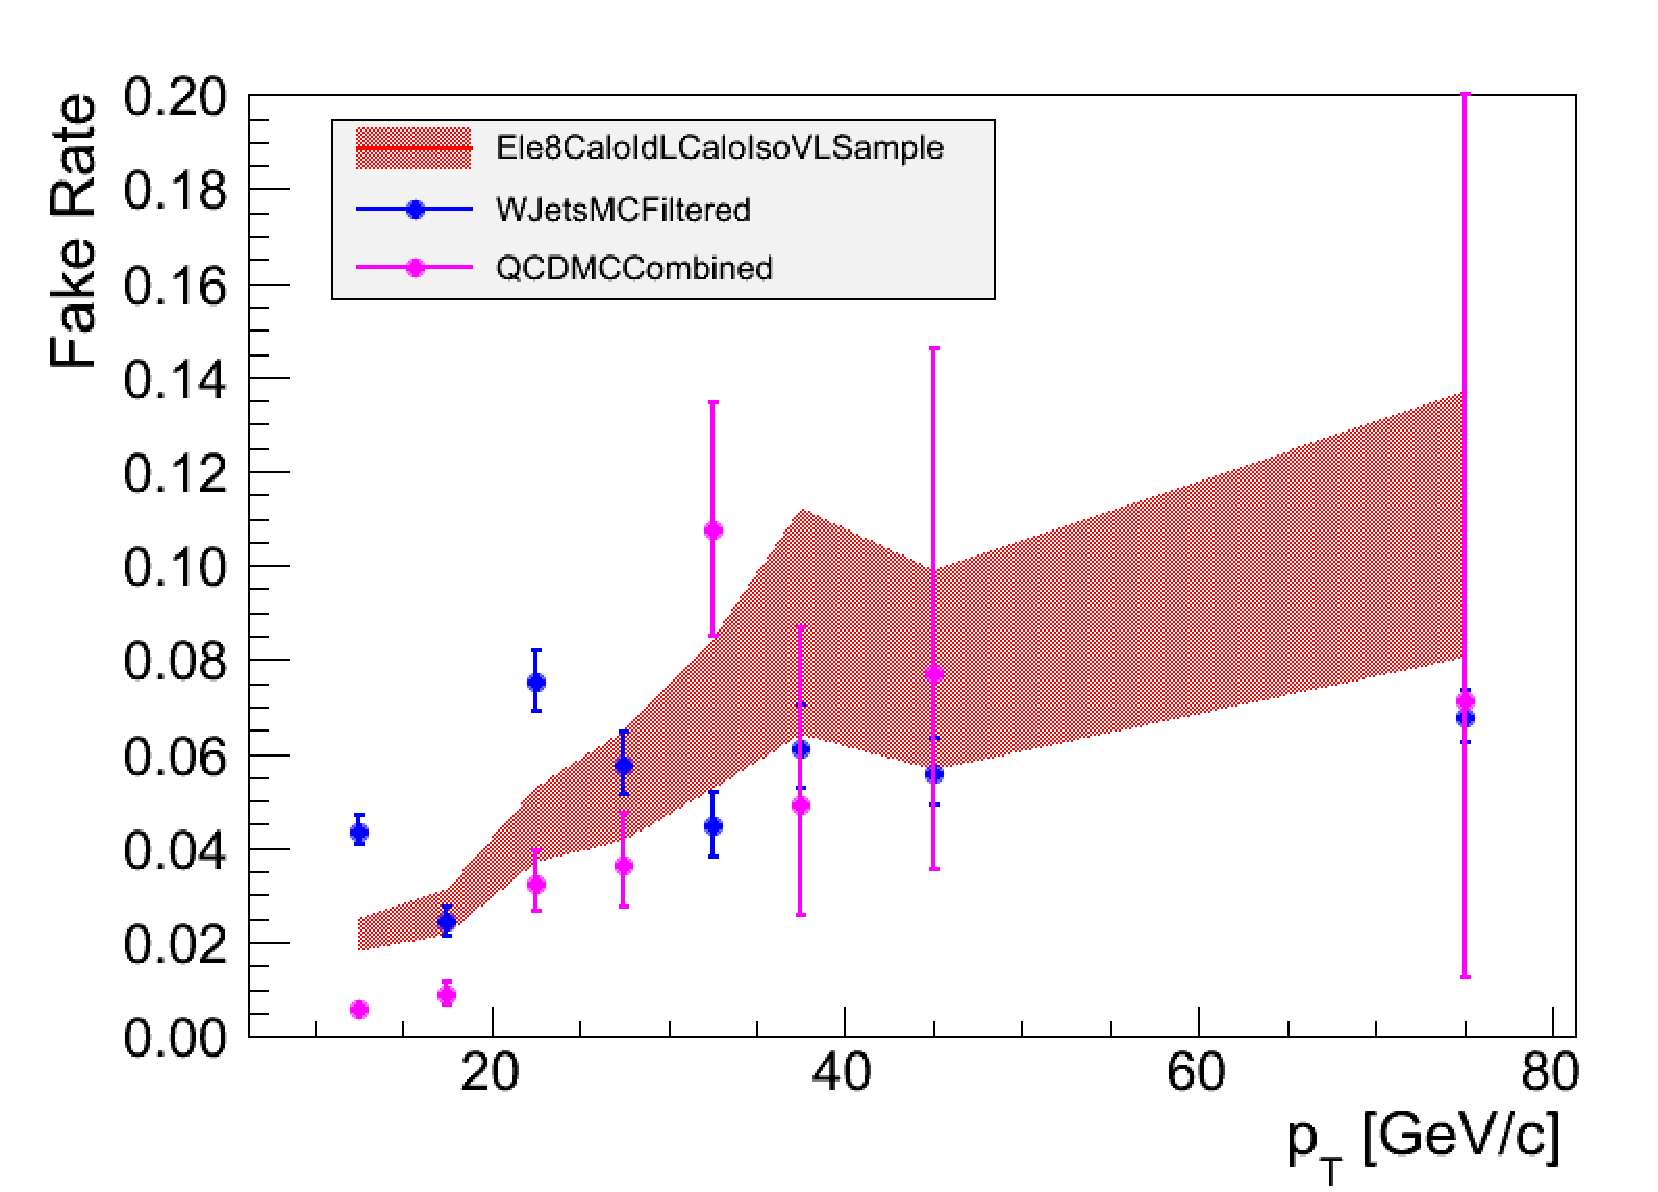
\includegraphics[width=0.45\textwidth]{figures/ElectronFakeRate_DenominatorV1_ptThreshold30_Pt.pdf}
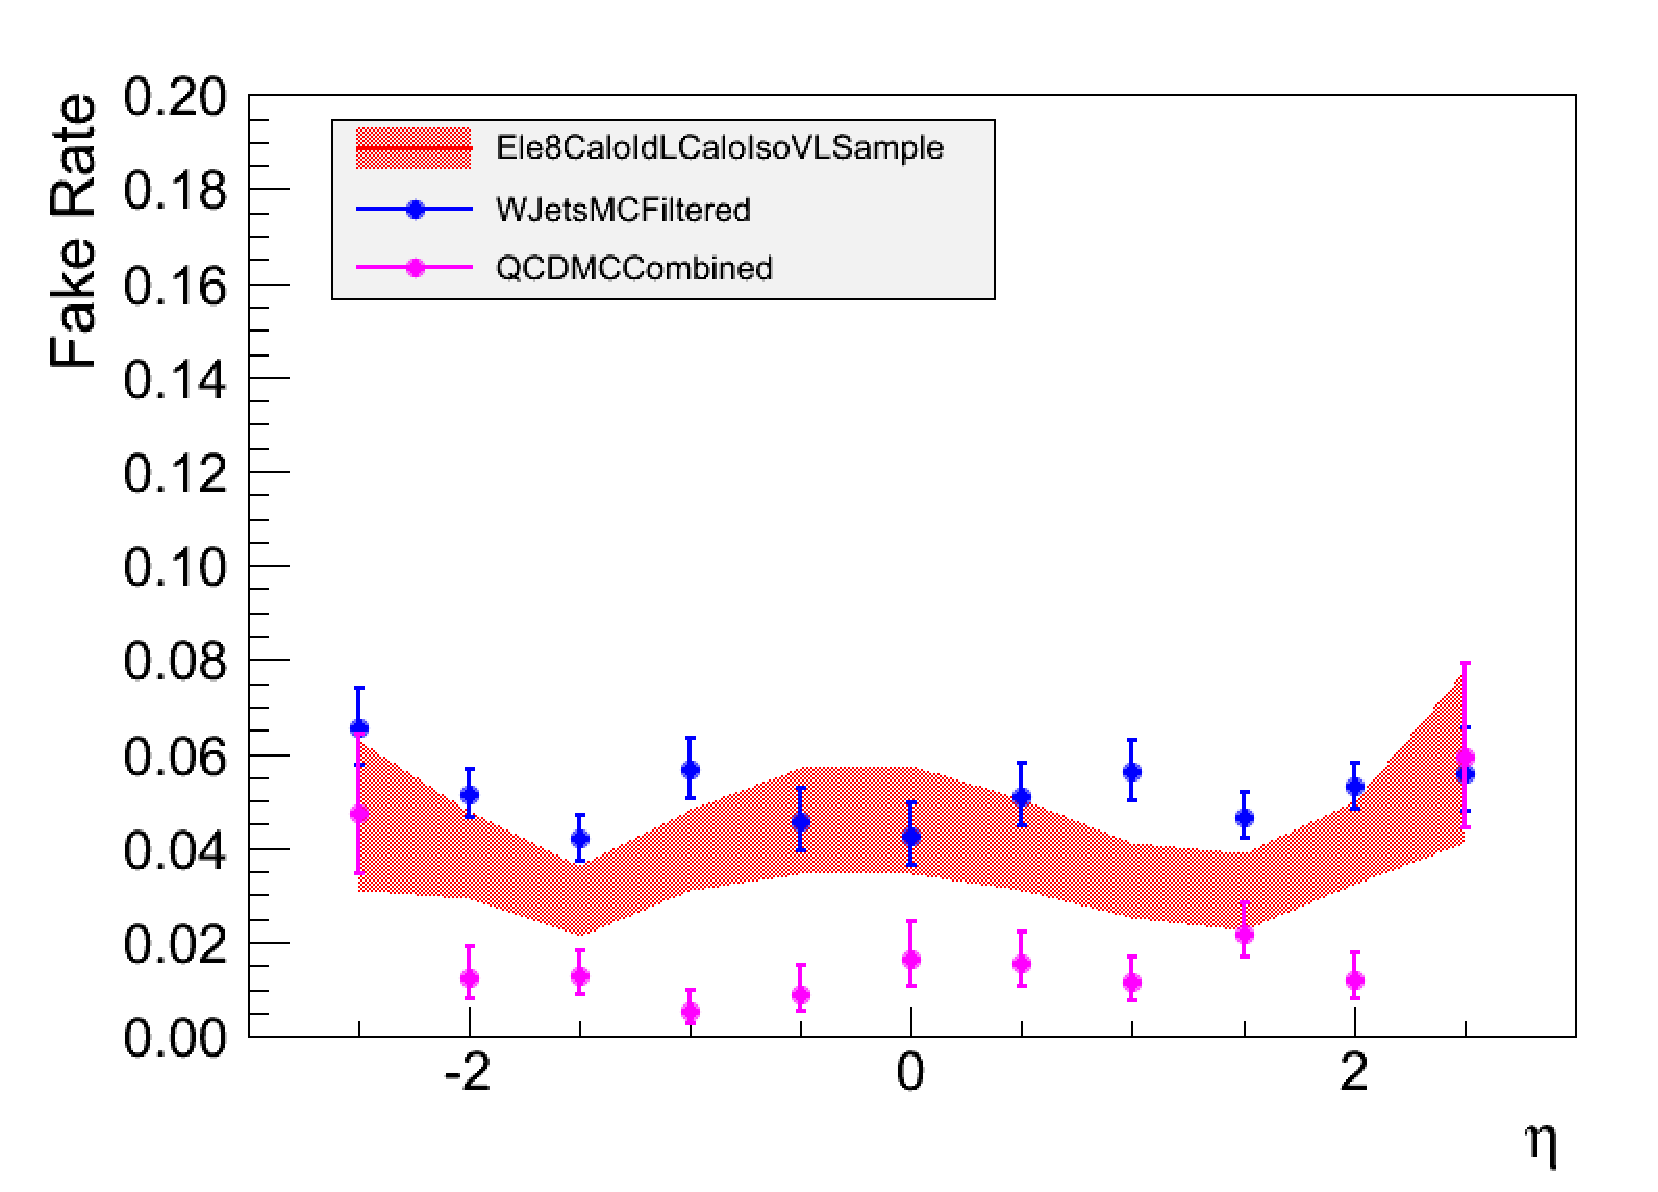
\includegraphics[width=0.45\textwidth]{figures/ElectronFakeRate_DenominatorV1_ptThreshold30_Eta.pdf}
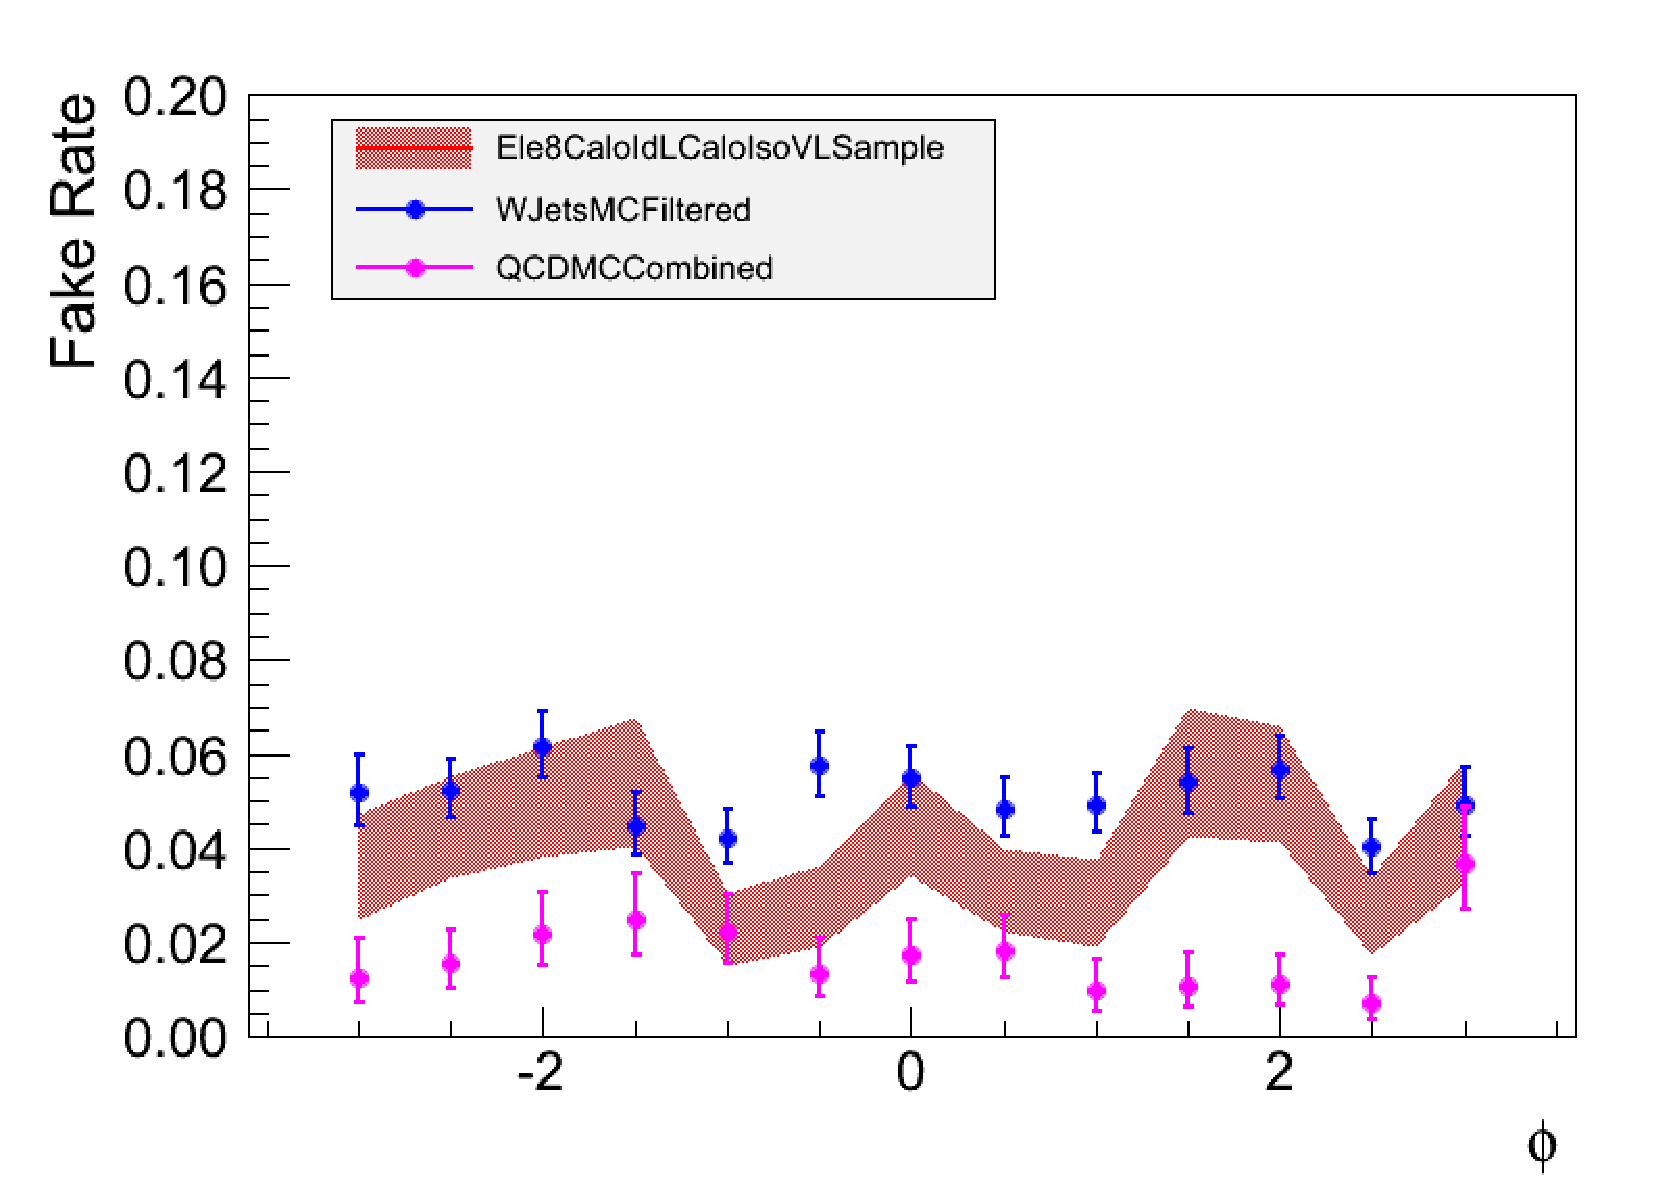
\includegraphics[width=0.45\textwidth]{figures/ElectronFakeRate_DenominatorV1_ptThreshold30_Phi.pdf}
\caption{Fake rates for V1 definition as a function of $p_T$,$\eta$, and $\phi$.}
\label{fig:ele_fr_V1_jet30}
\end{center}
\end{figure}

\begin{figure}[!htbp]
\begin{center}
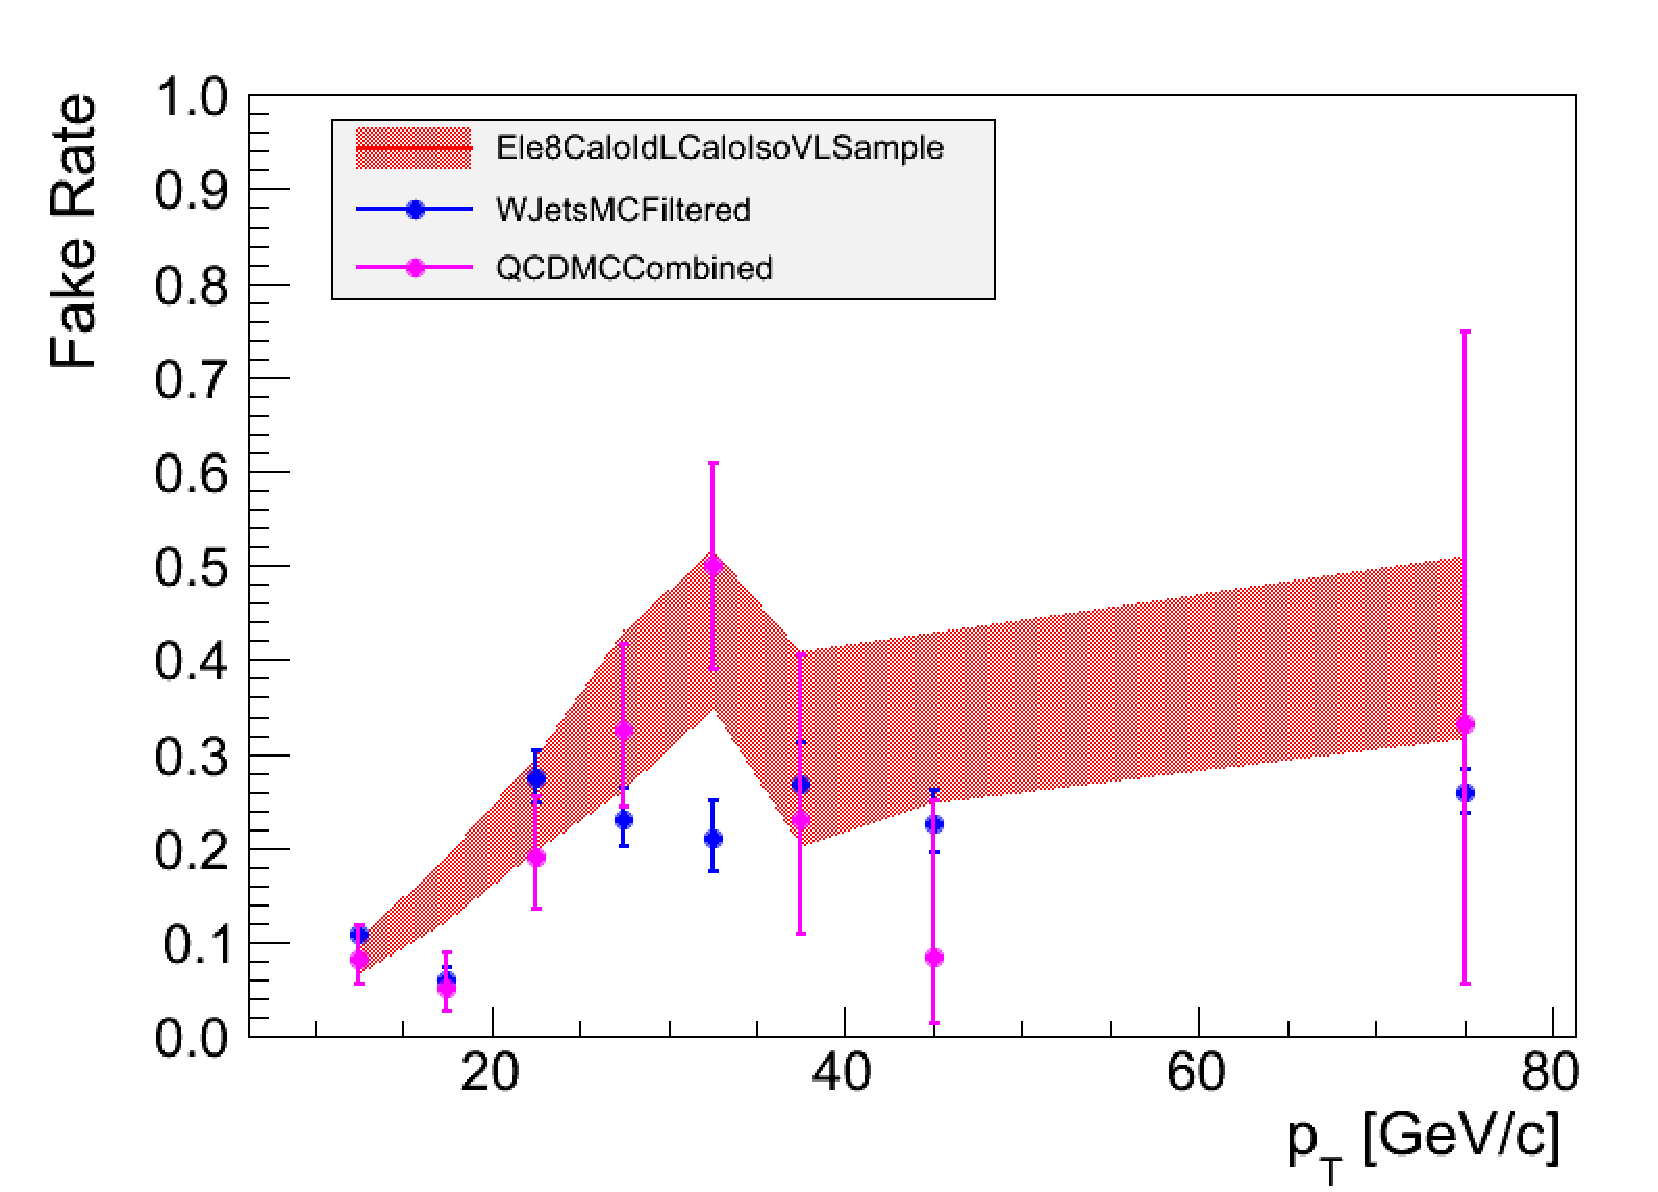
\includegraphics[width=0.45\textwidth]{figures/ElectronFakeRate_DenominatorV2_ptThreshold30_Pt.pdf}
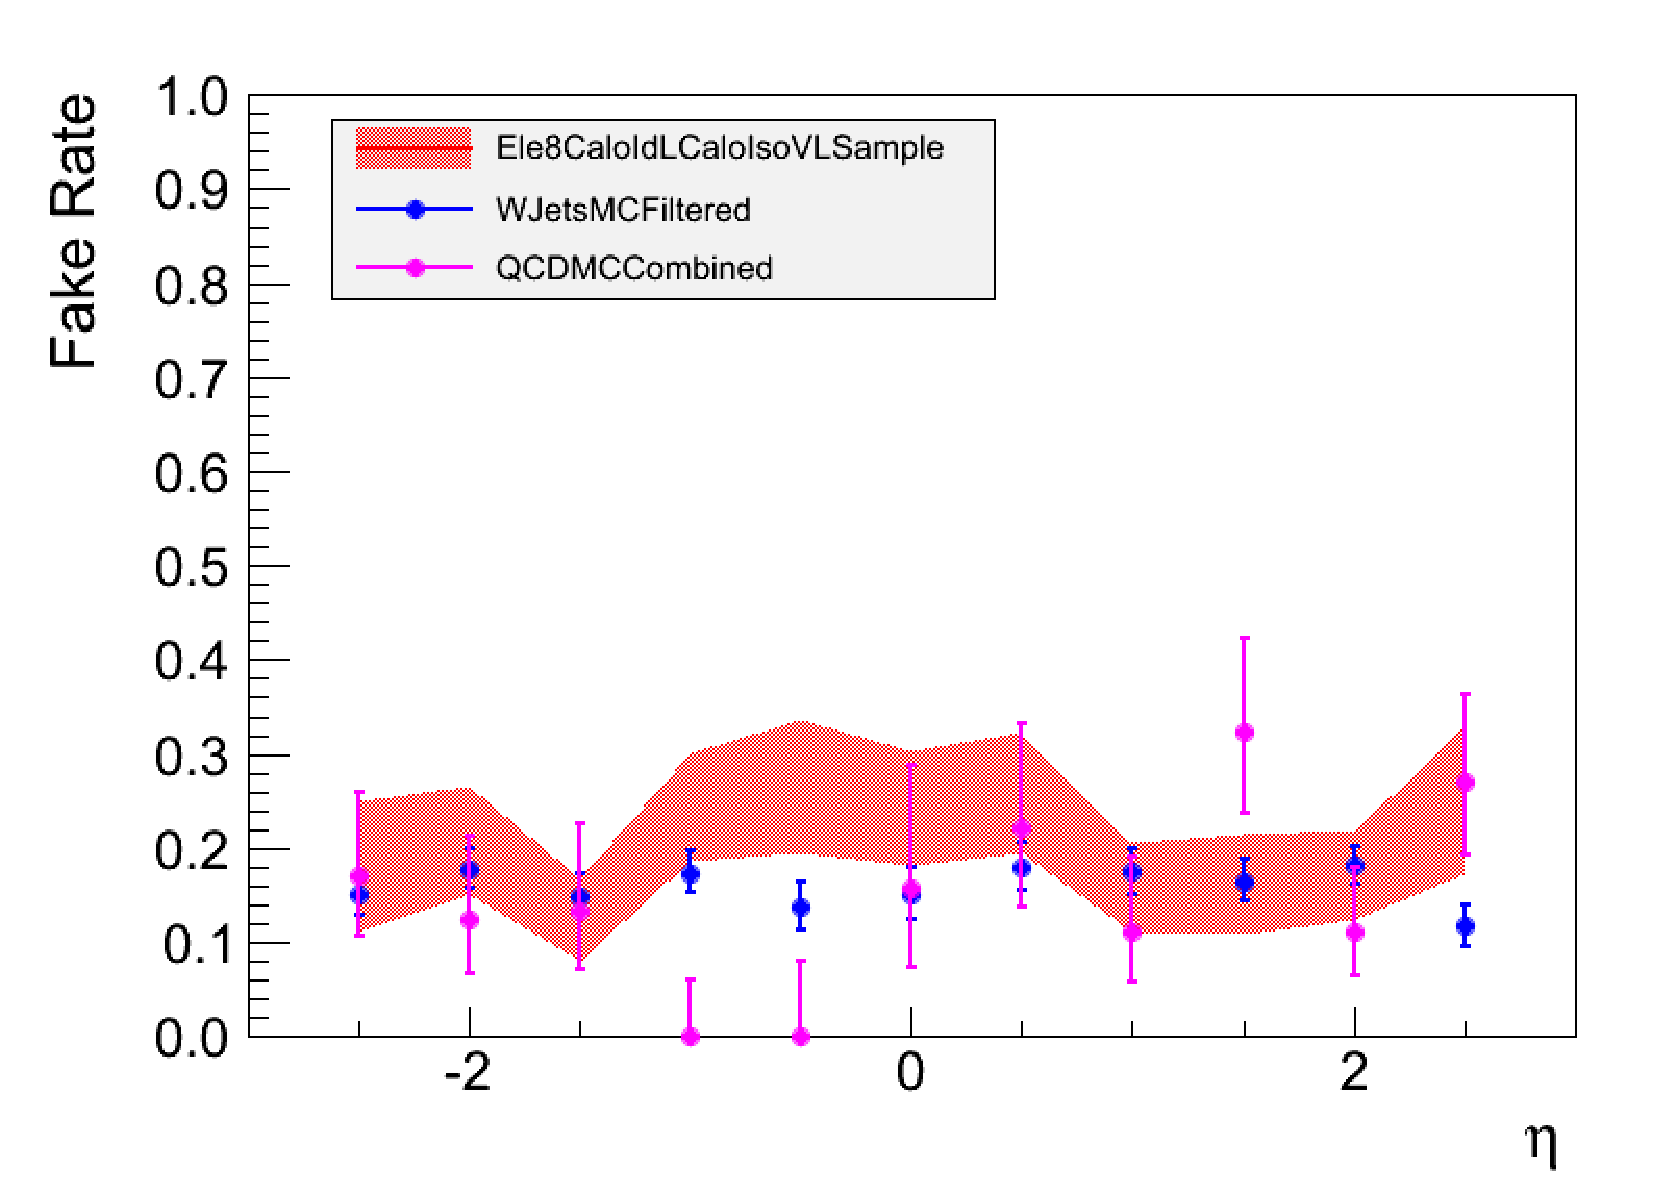
\includegraphics[width=0.45\textwidth]{figures/ElectronFakeRate_DenominatorV2_ptThreshold30_Eta.pdf}
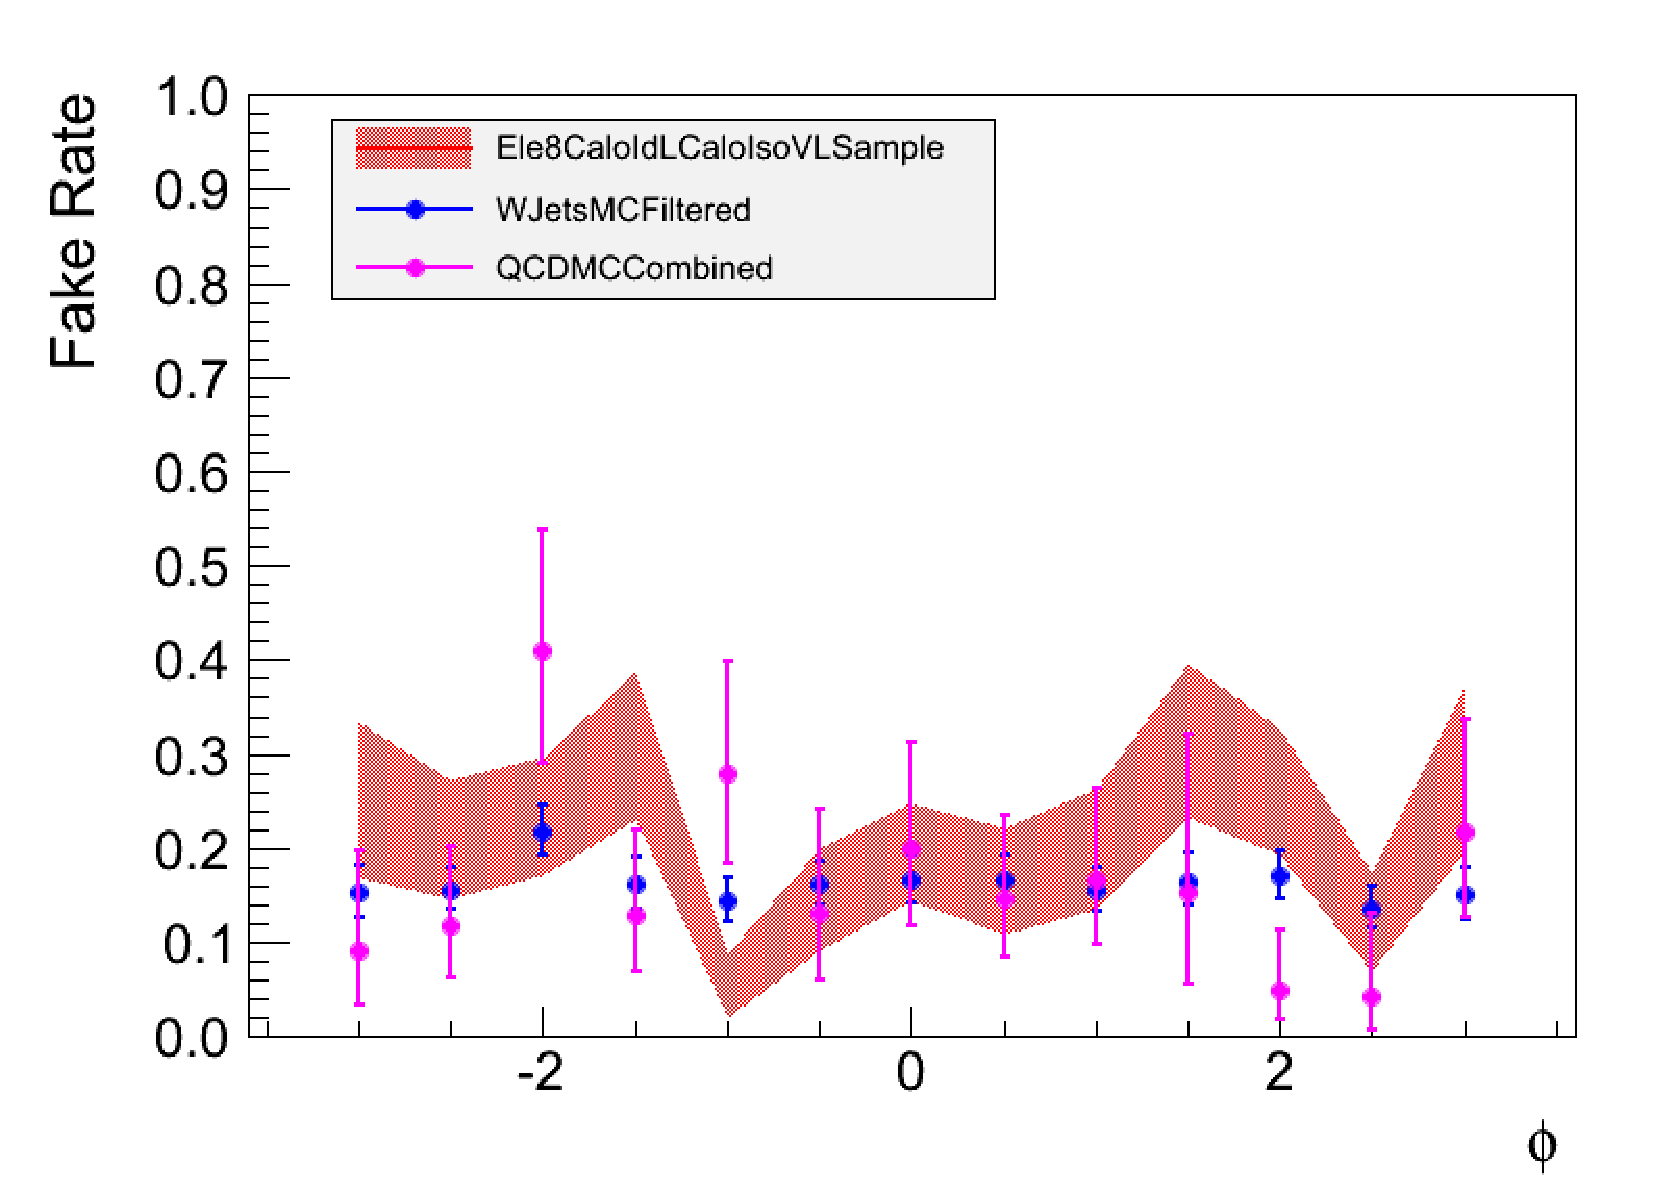
\includegraphics[width=0.45\textwidth]{figures/ElectronFakeRate_DenominatorV2_ptThreshold30_Phi.pdf}
\caption{Fake rates for V2 definition as a function of $p_T$,$\eta$, and $\phi$.}
\label{fig:ele_fr_V2_jet30}
\end{center}
\end{figure}

\begin{figure}[!htbp]
\begin{center}
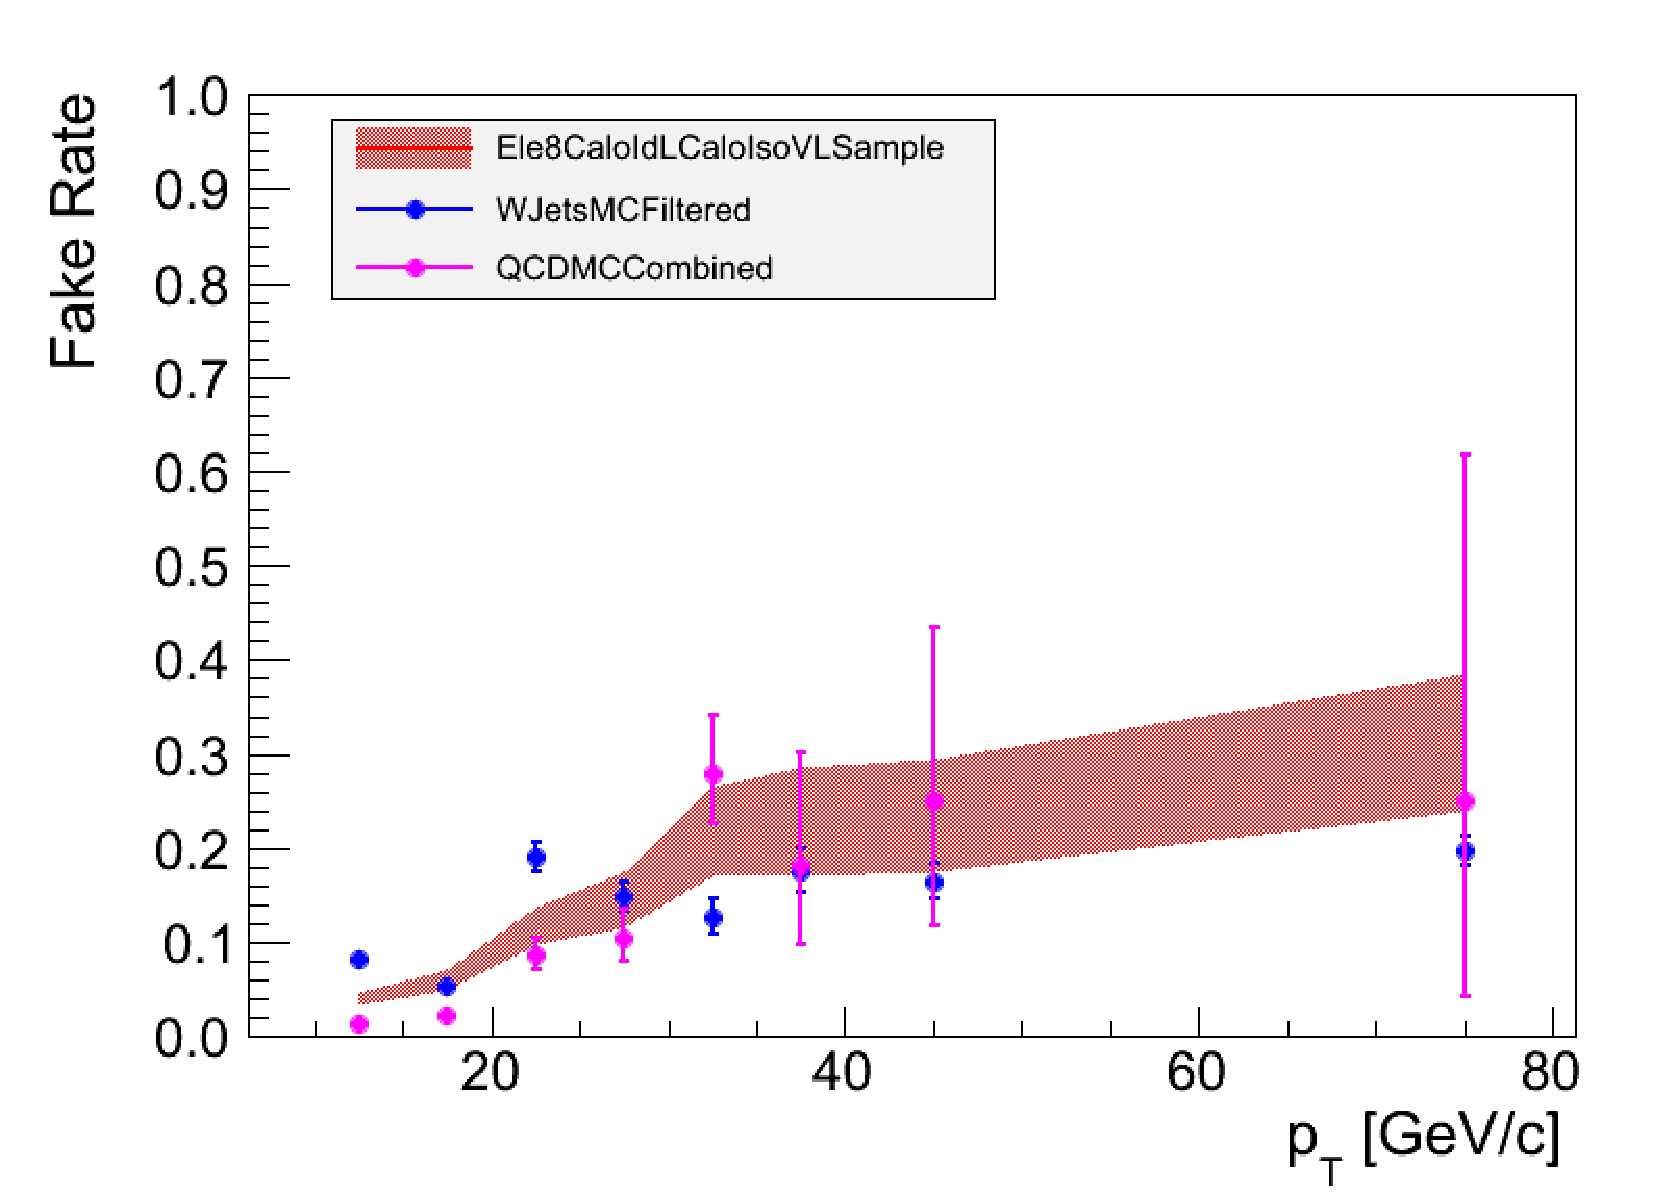
\includegraphics[width=0.45\textwidth]{figures/ElectronFakeRate_DenominatorV3_ptThreshold30_Pt.pdf}
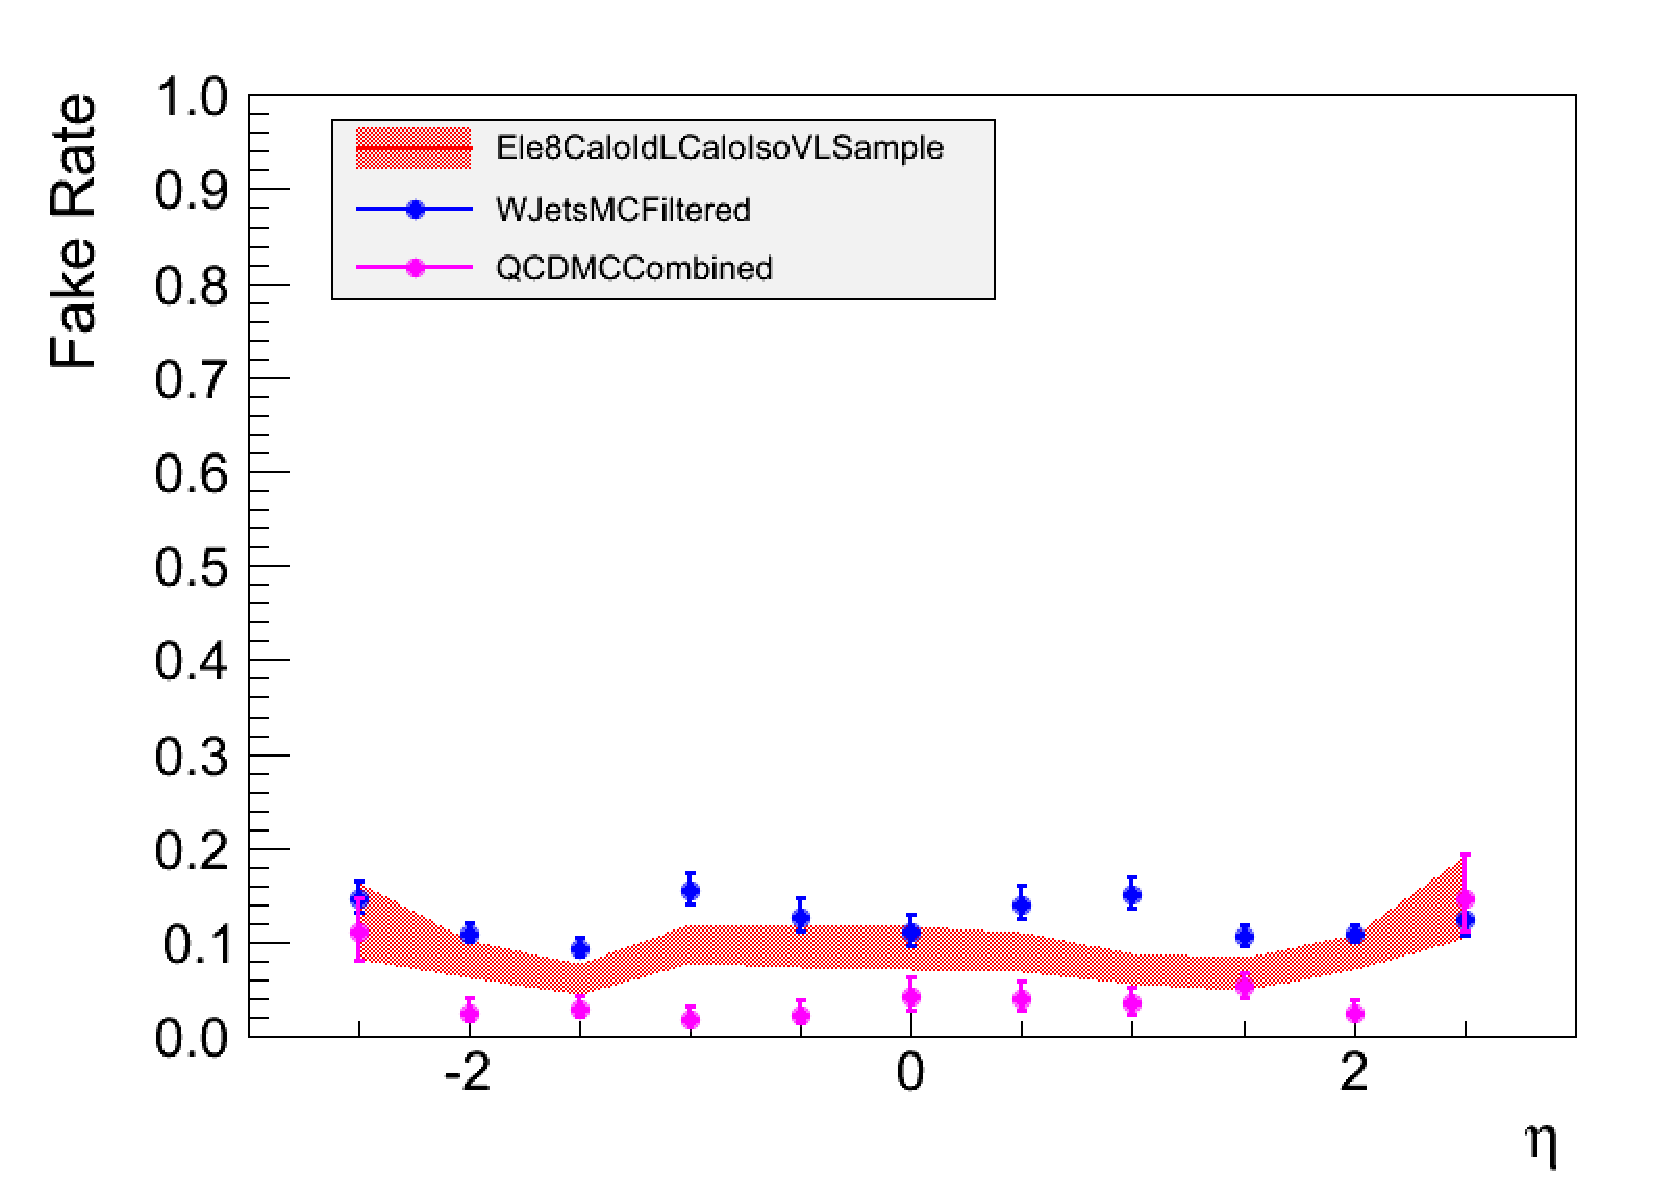
\includegraphics[width=0.45\textwidth]{figures/ElectronFakeRate_DenominatorV3_ptThreshold30_Eta.pdf}
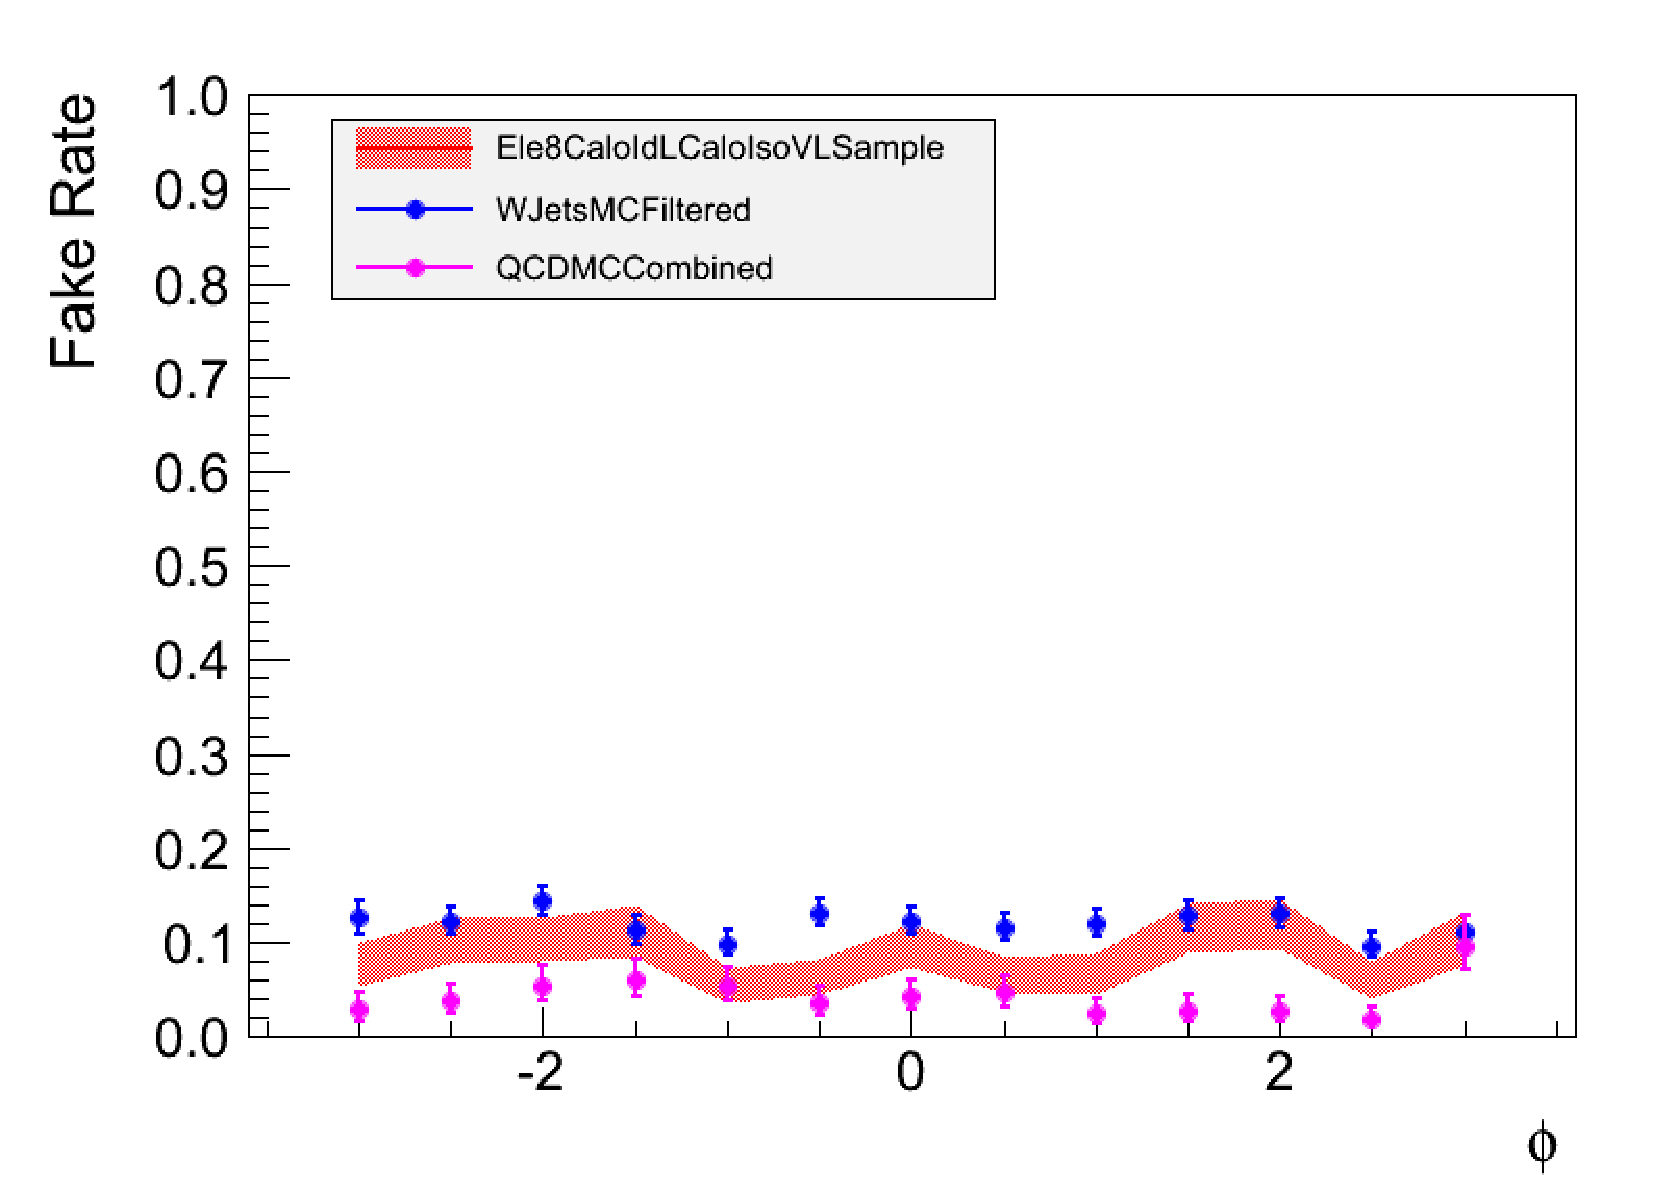
\includegraphics[width=0.45\textwidth]{figures/ElectronFakeRate_DenominatorV3_ptThreshold30_Phi.pdf}
\caption{Fake rates for V3 definition as a function of $p_T$,$\eta$, and $\phi$.}
\label{fig:ele_fr_V3_jet30}
\end{center}
\end{figure}

\begin{figure}[!htbp]
\begin{center}
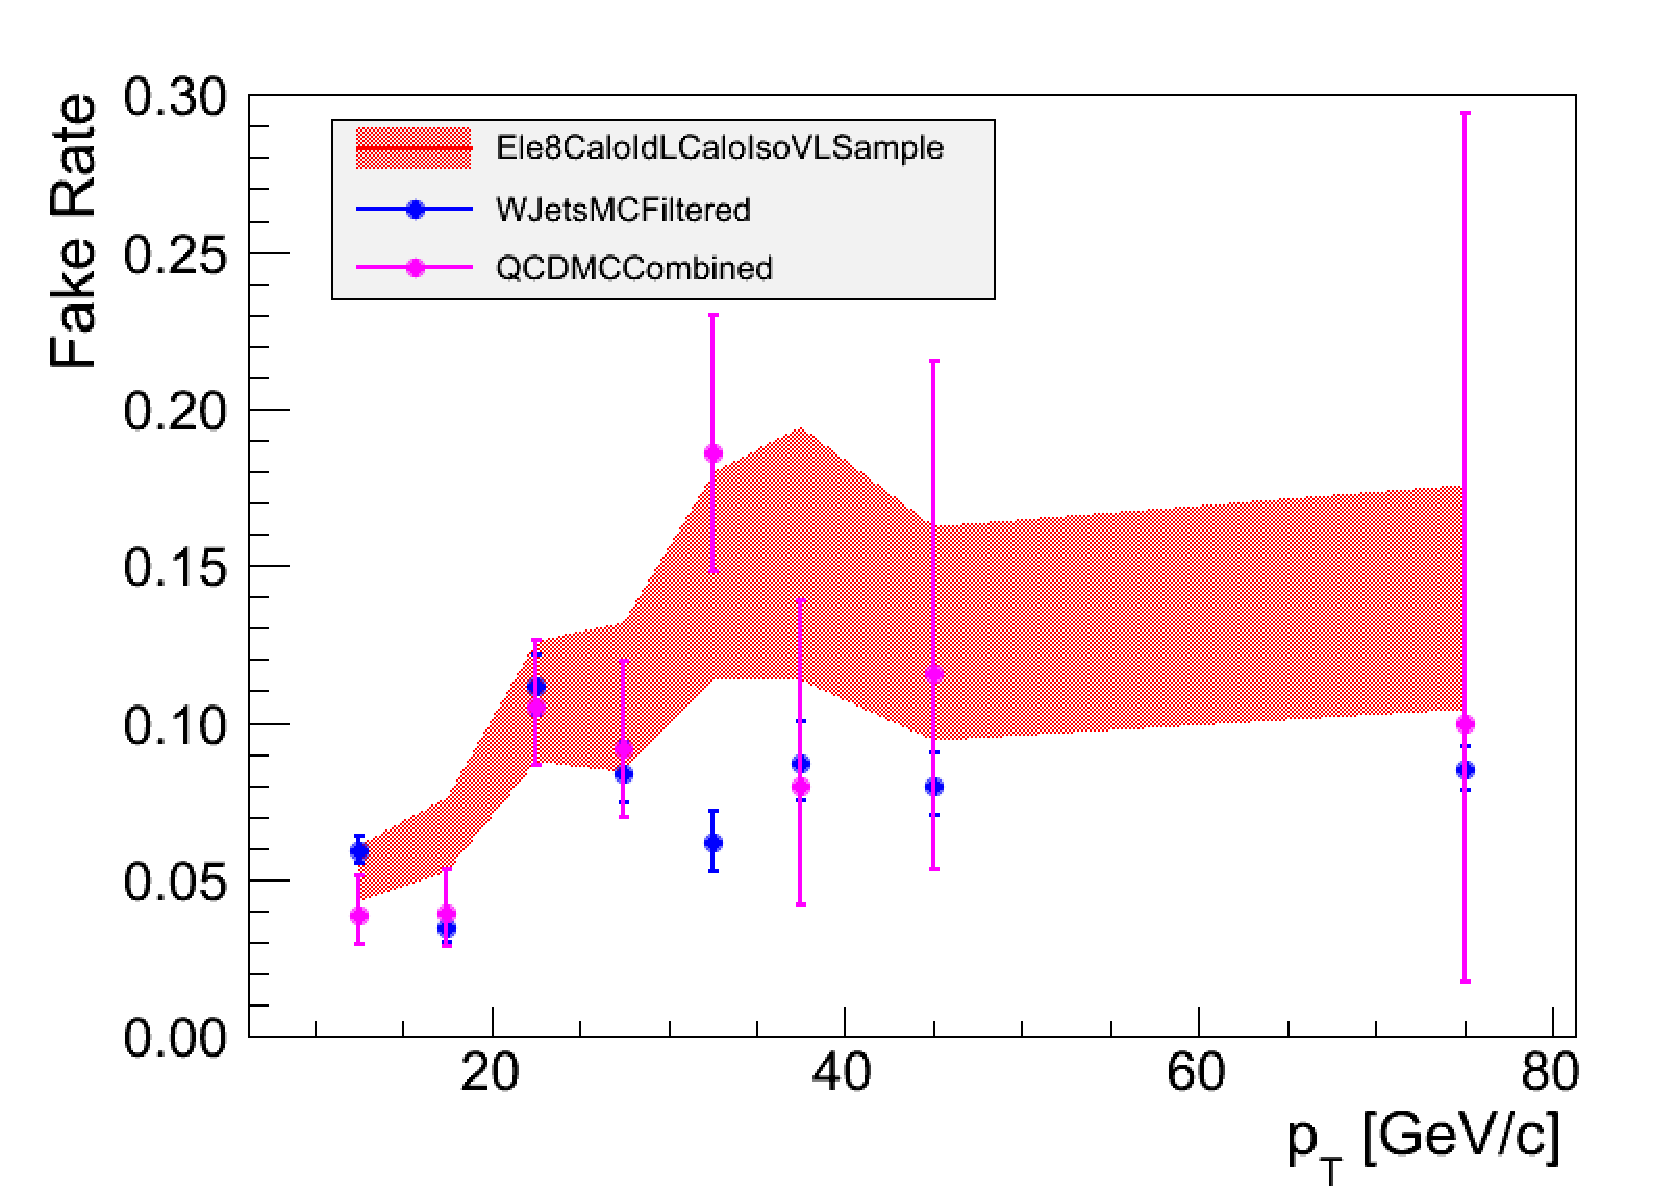
\includegraphics[width=0.45\textwidth]{figures/ElectronFakeRate_DenominatorV4_ptThreshold30_Pt.pdf}
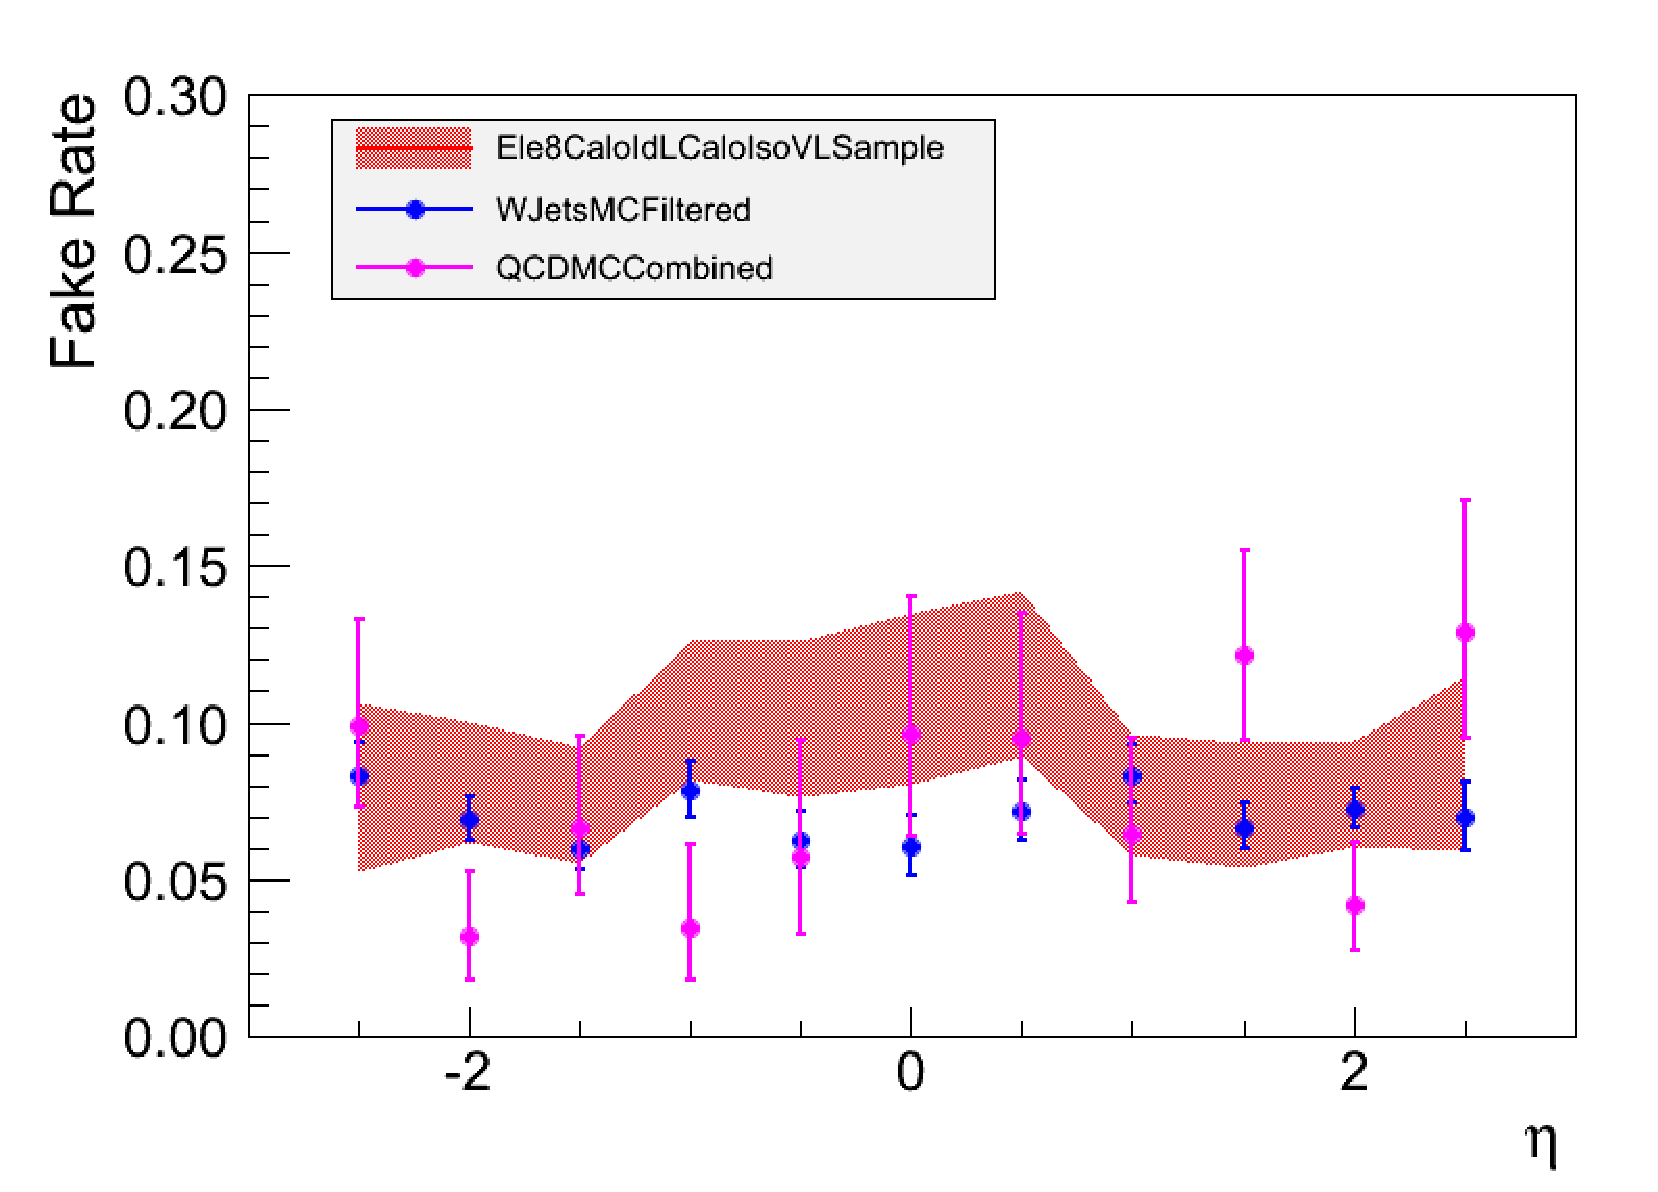
\includegraphics[width=0.45\textwidth]{figures/ElectronFakeRate_DenominatorV4_ptThreshold30_Eta.pdf}
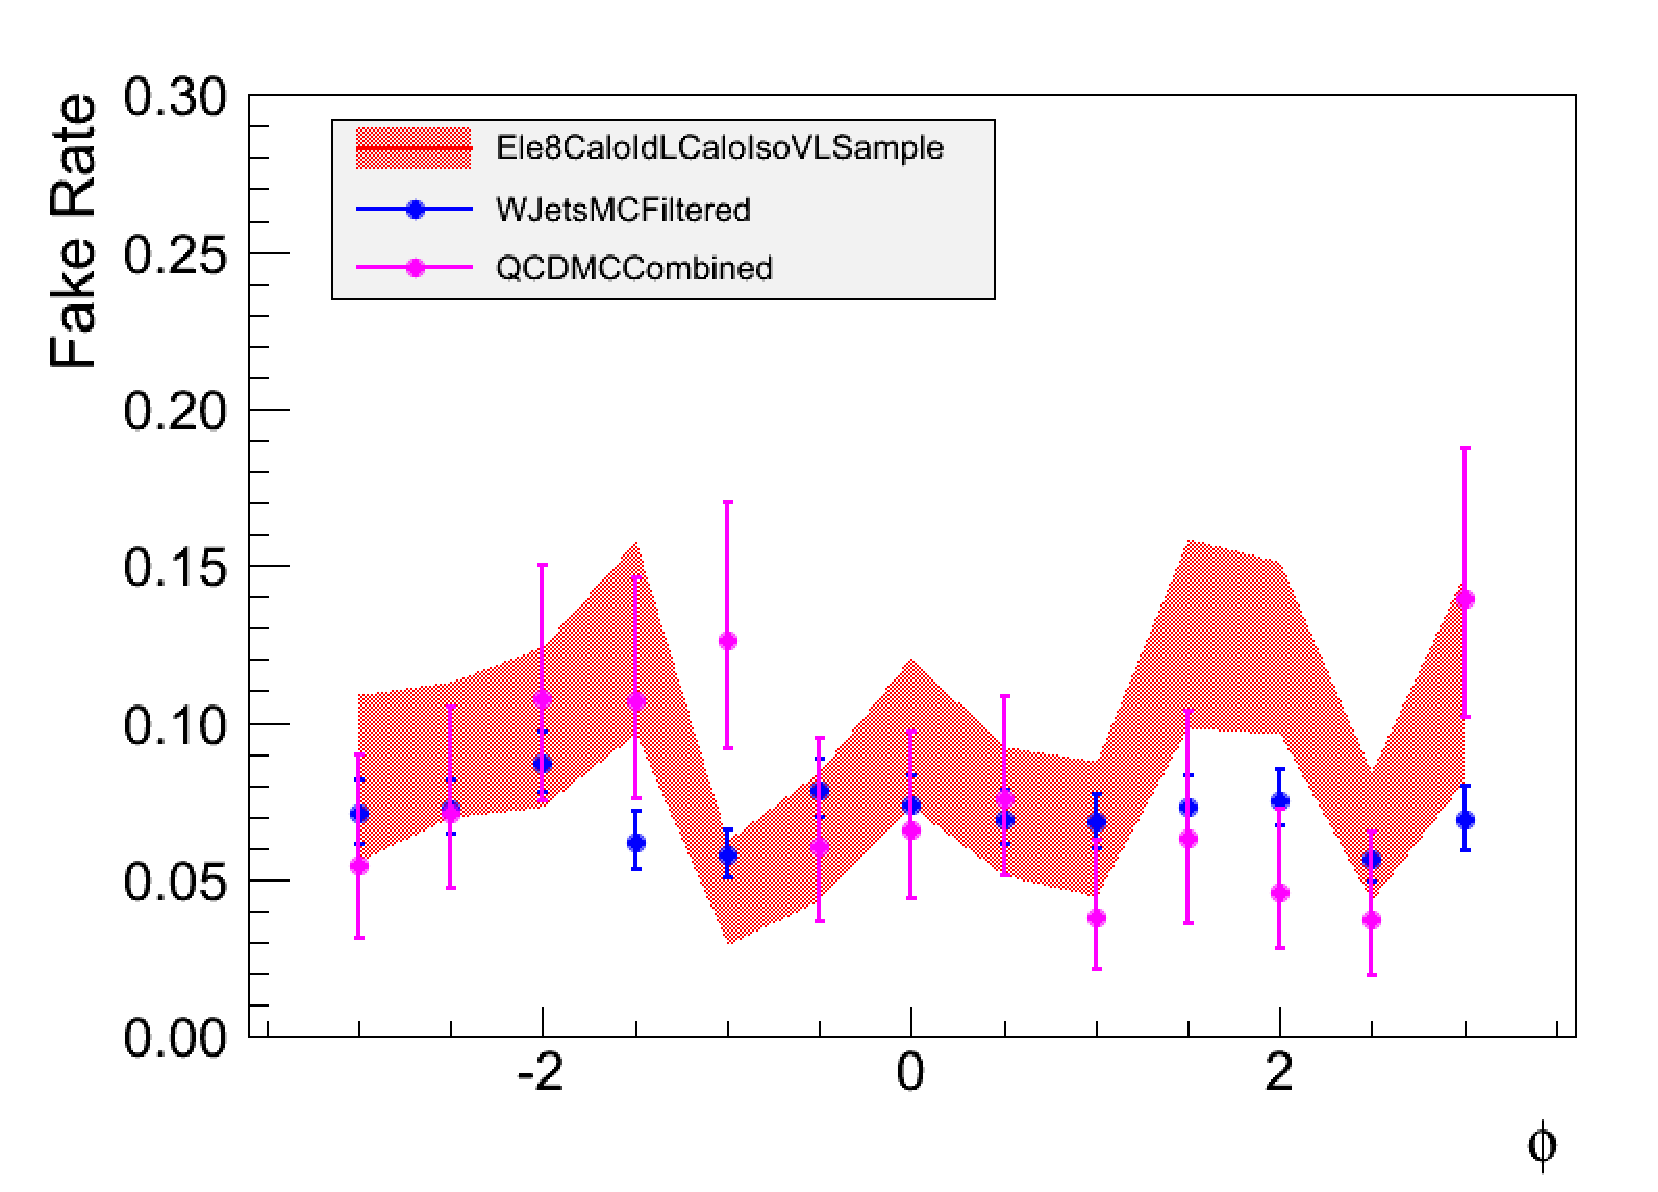
\includegraphics[width=0.45\textwidth]{figures/ElectronFakeRate_DenominatorV4_ptThreshold30_Phi.pdf}
\caption{Fake rates for V4 definition as a function of $p_T$,$\eta$, and $\phi$.}
\label{fig:ele_fr_V4_jet30}
\end{center}
\end{figure}

Due to the fact that the Monte Carlo simulation does not have an implementation of the trigger used
to collect the fake electron candidates, it is expected that the Monte Carlo fake rate will differ
from the data fake rates. The V2 fake rate is expected to give better agreement between data and 
Monte Carlo simulation, since the denominator is already fully isolated. For $p_{T} > 20$ GeV, 
the fake rate from QCD Monte Carlo actually gives a reasonable description of the data. The difference
between the QCD Monte Carlo and the W+Jet Monte Carlo fake rate reflects the systematic uncertainties
due to different fake composition.


\subsubsection{Systematics}
To study the systematic uncertainty due to the jet $p_{T}$ spectrum, we compare the fake rates
measured requiring different thresholds on the $p_{T}$ of the leading jet. The comparisons
are shown in Fig \ref{fig:ele_fr_jetPtThresholdDependence} for the different denominator definitions. 


\begin{figure}[!htbp]
\begin{center}
\subfigure[V1 Denominator]{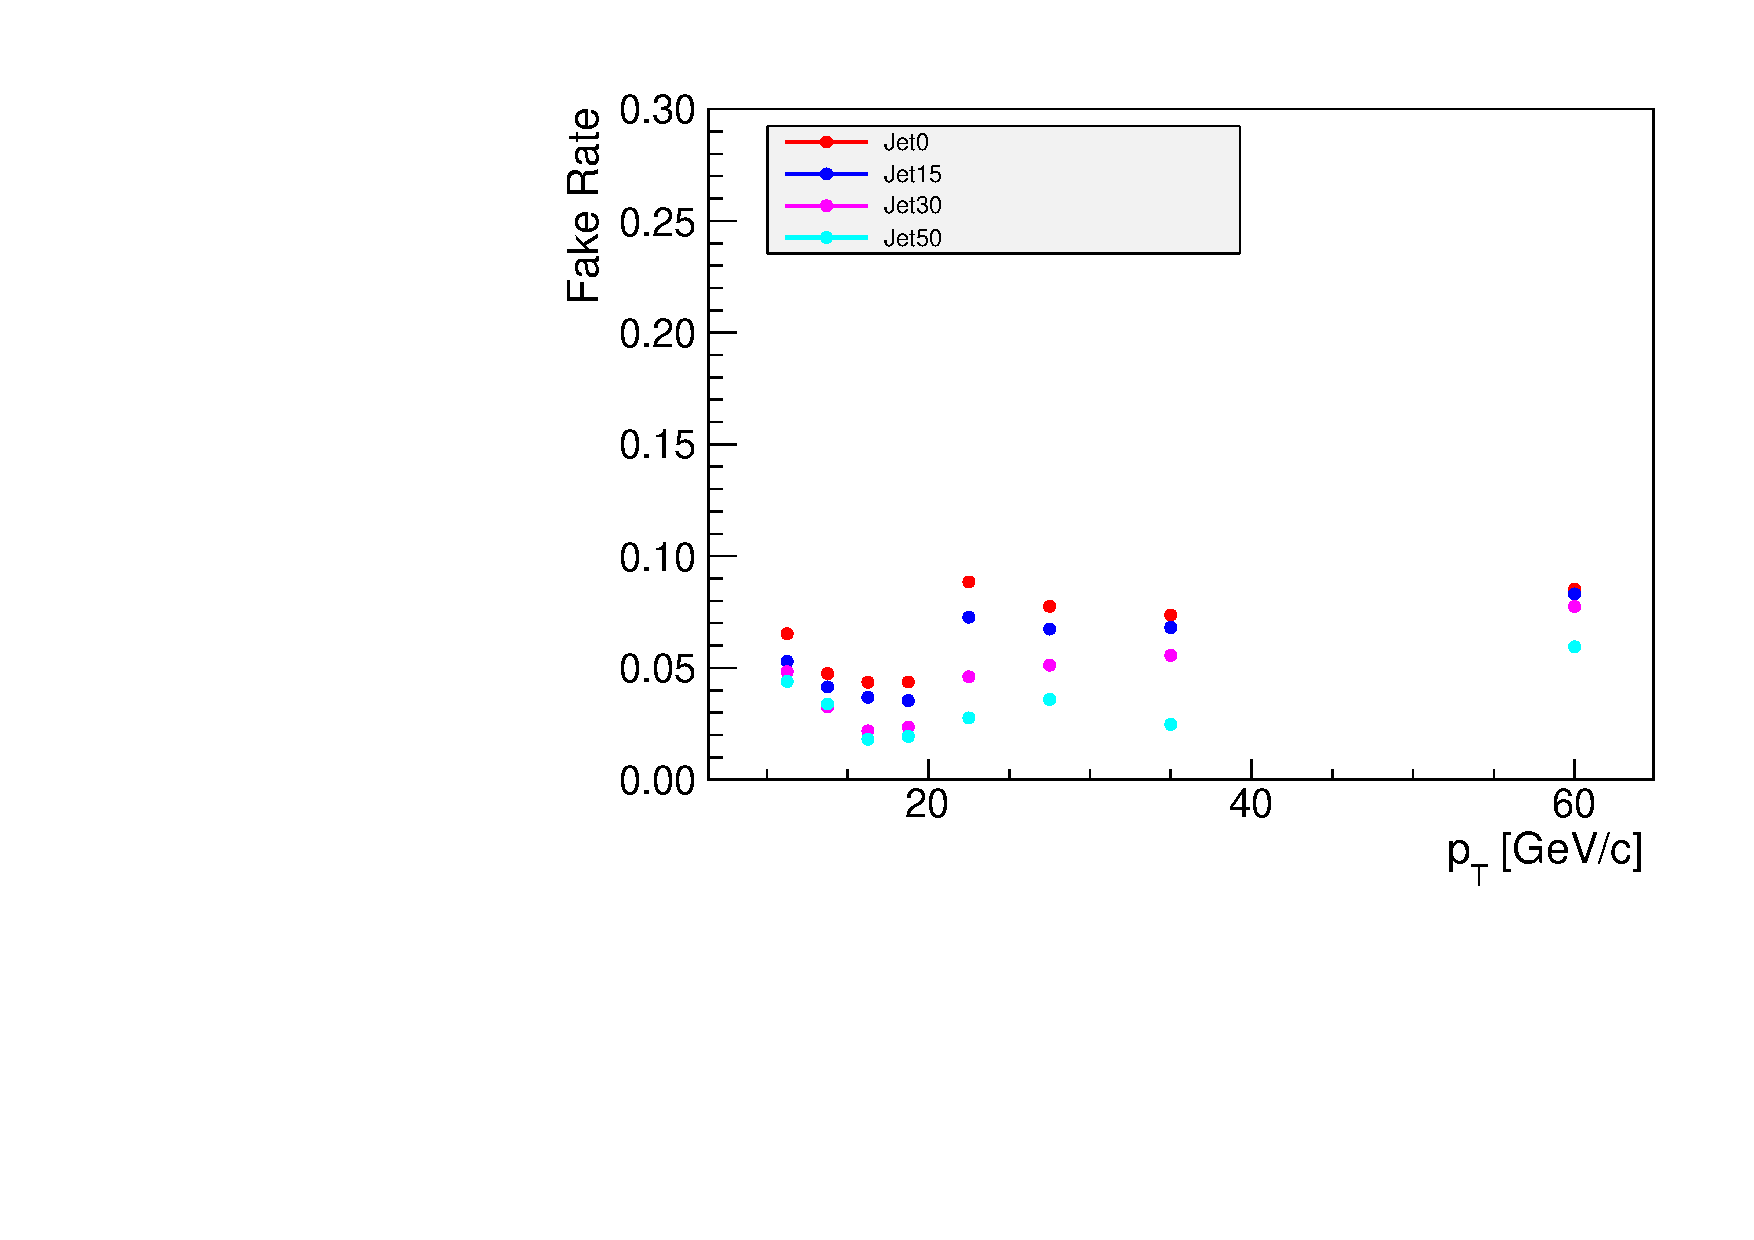
\includegraphics[width=0.45\textwidth]{figures/ElectronFakeRate_DenominatorV1_Ele8CaloIdLCaloIsoVLSample_Pt.pdf}}
\subfigure[V2 Denominator]{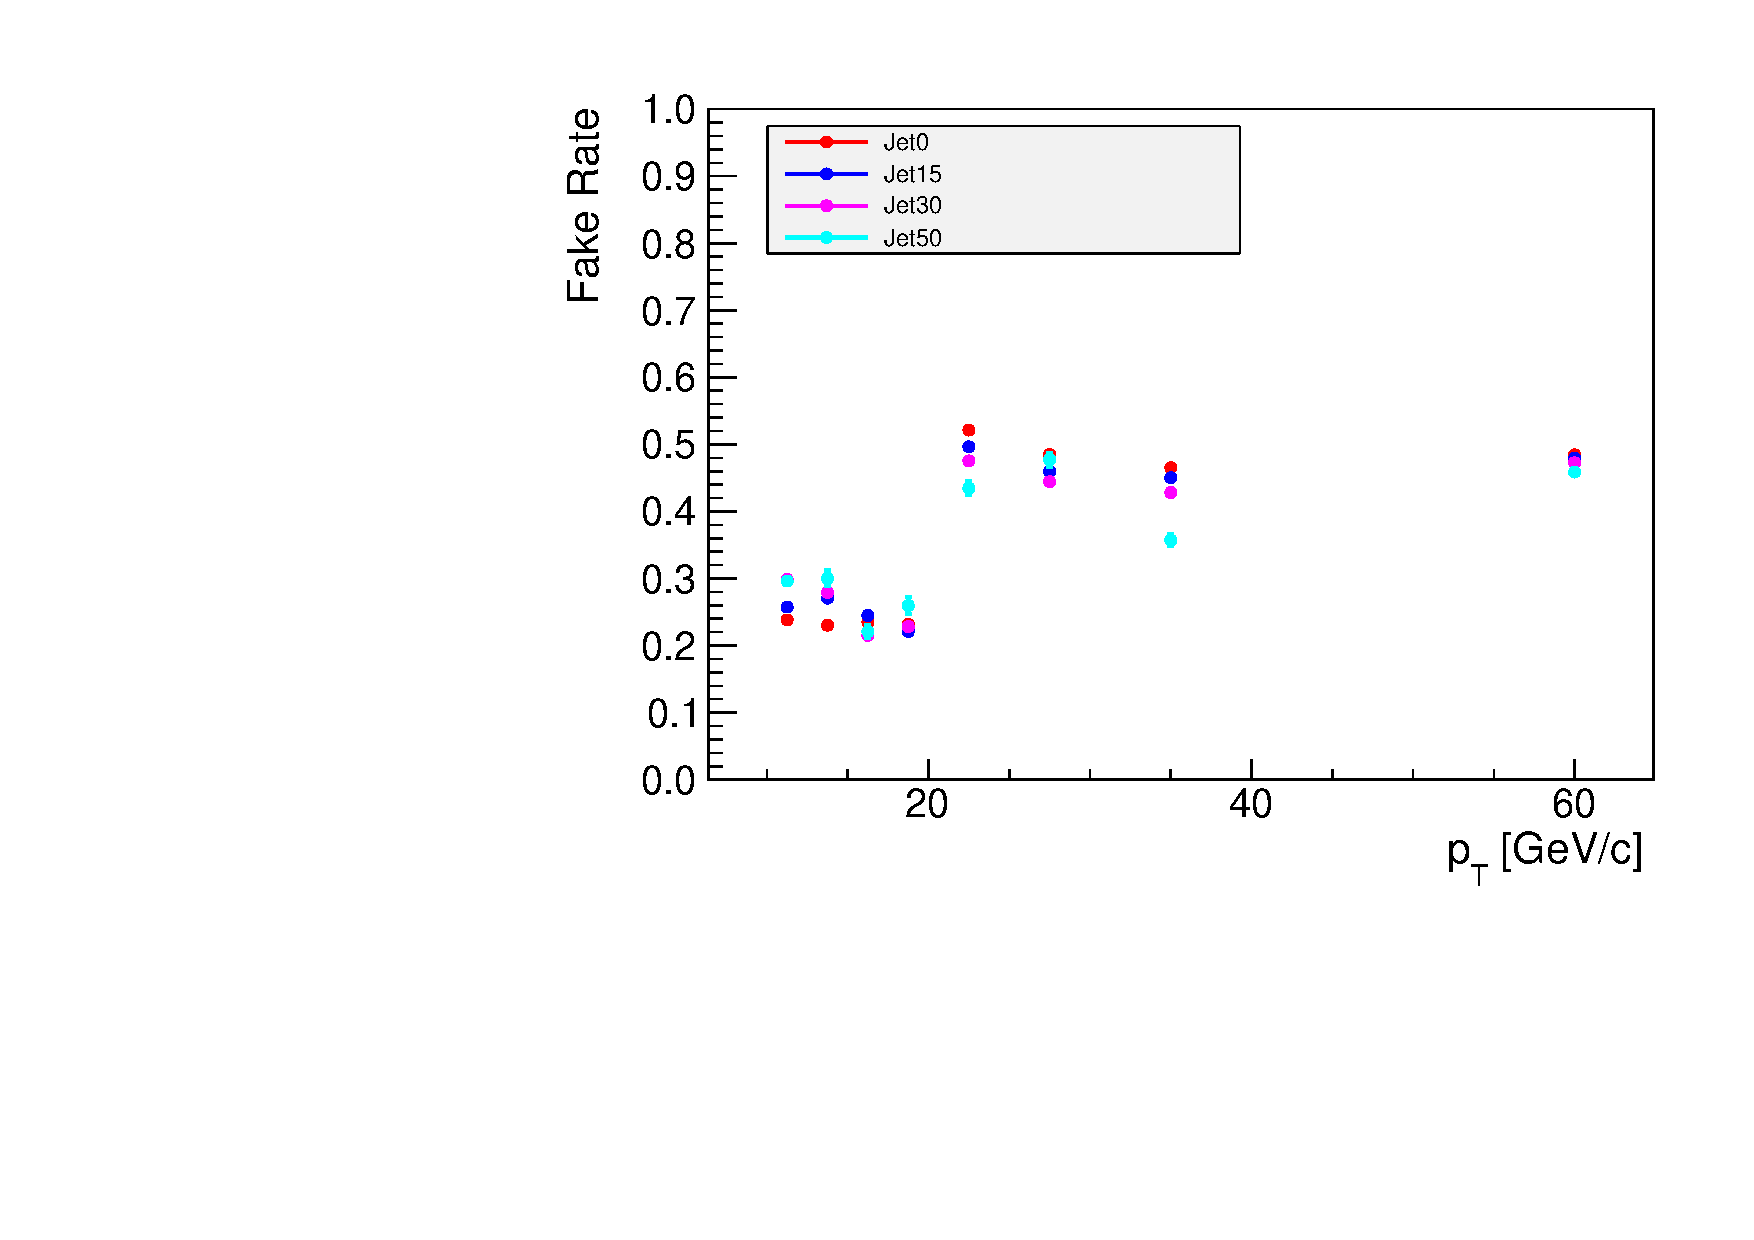
\includegraphics[width=0.45\textwidth]{figures/ElectronFakeRate_DenominatorV2_Ele8CaloIdLCaloIsoVLSample_Pt.pdf}}
\subfigure[V3 Denominator]{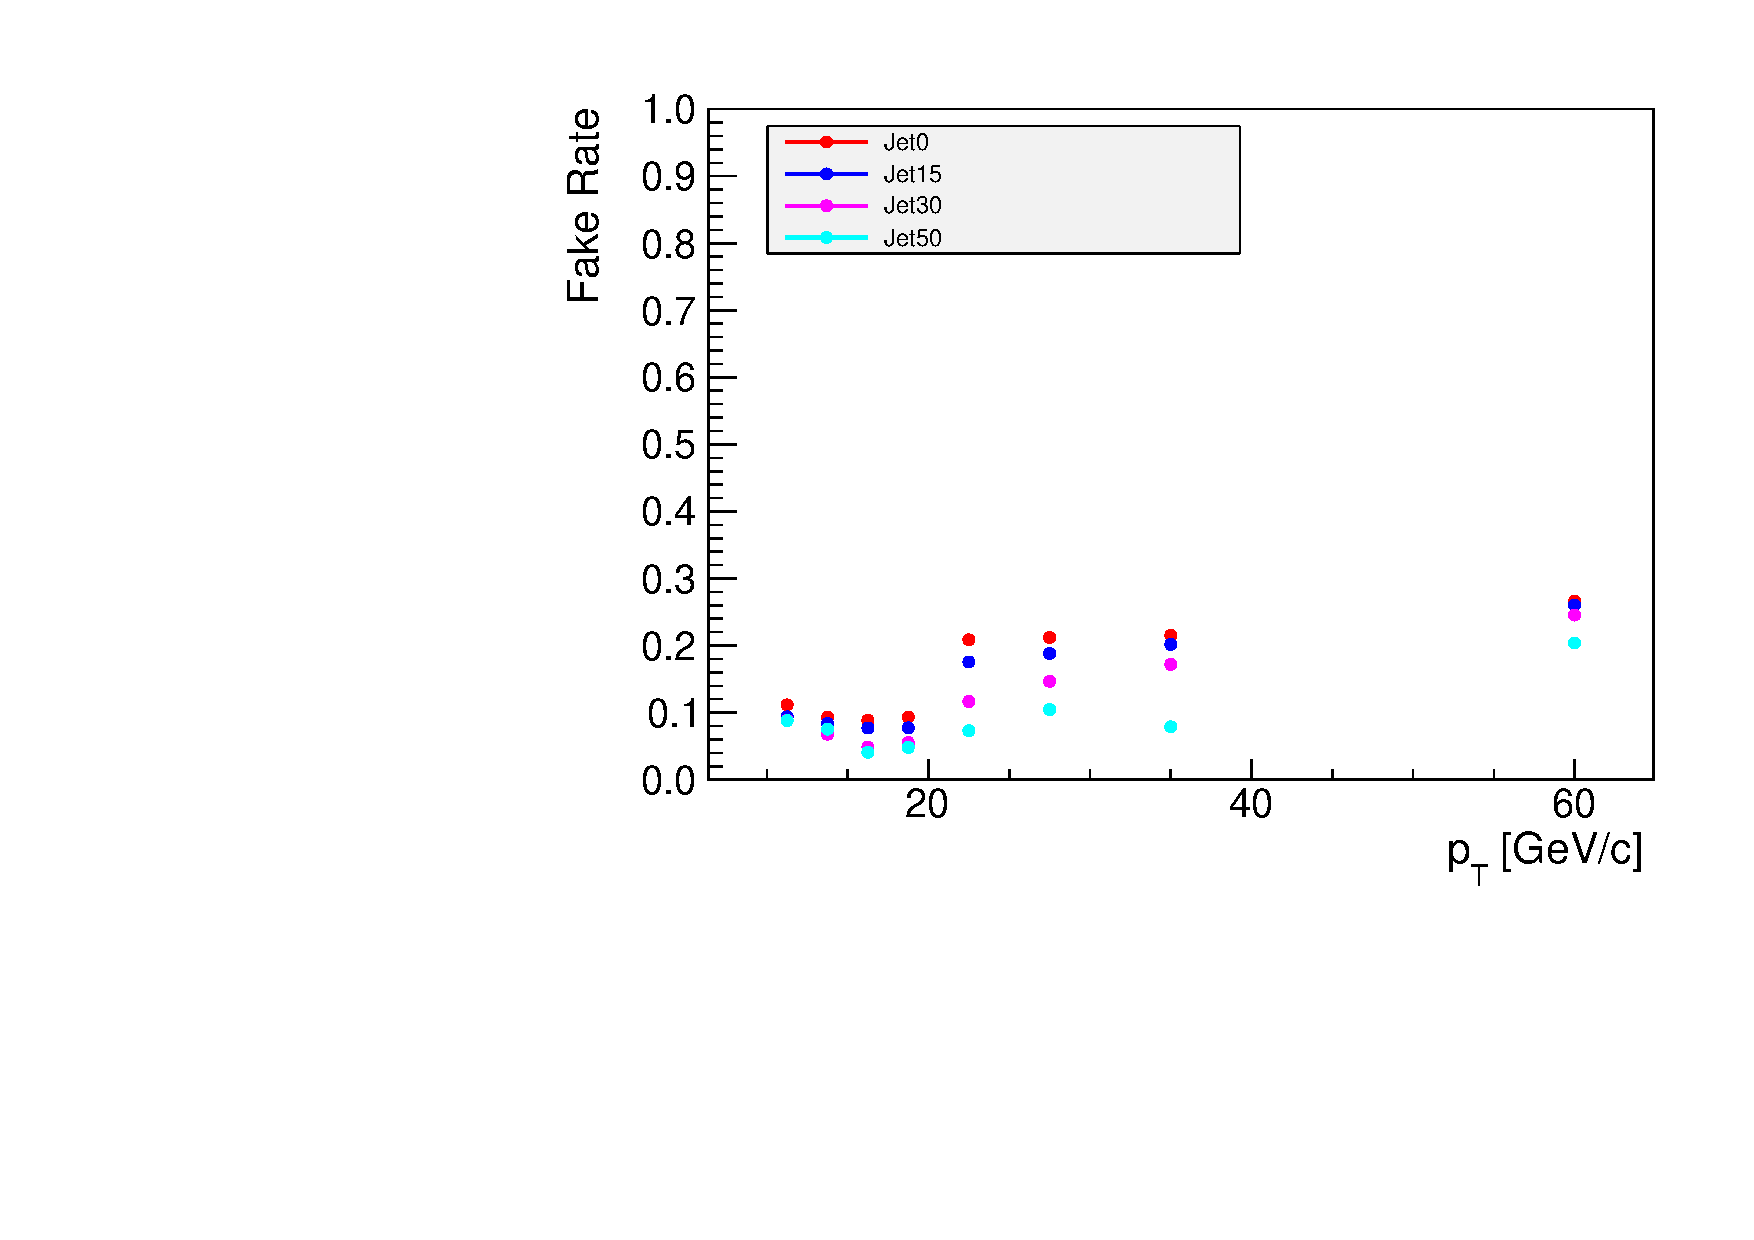
\includegraphics[width=0.45\textwidth]{figures/ElectronFakeRate_DenominatorV3_Ele8CaloIdLCaloIsoVLSample_Pt.pdf}}
\subfigure[V4 Denominator]{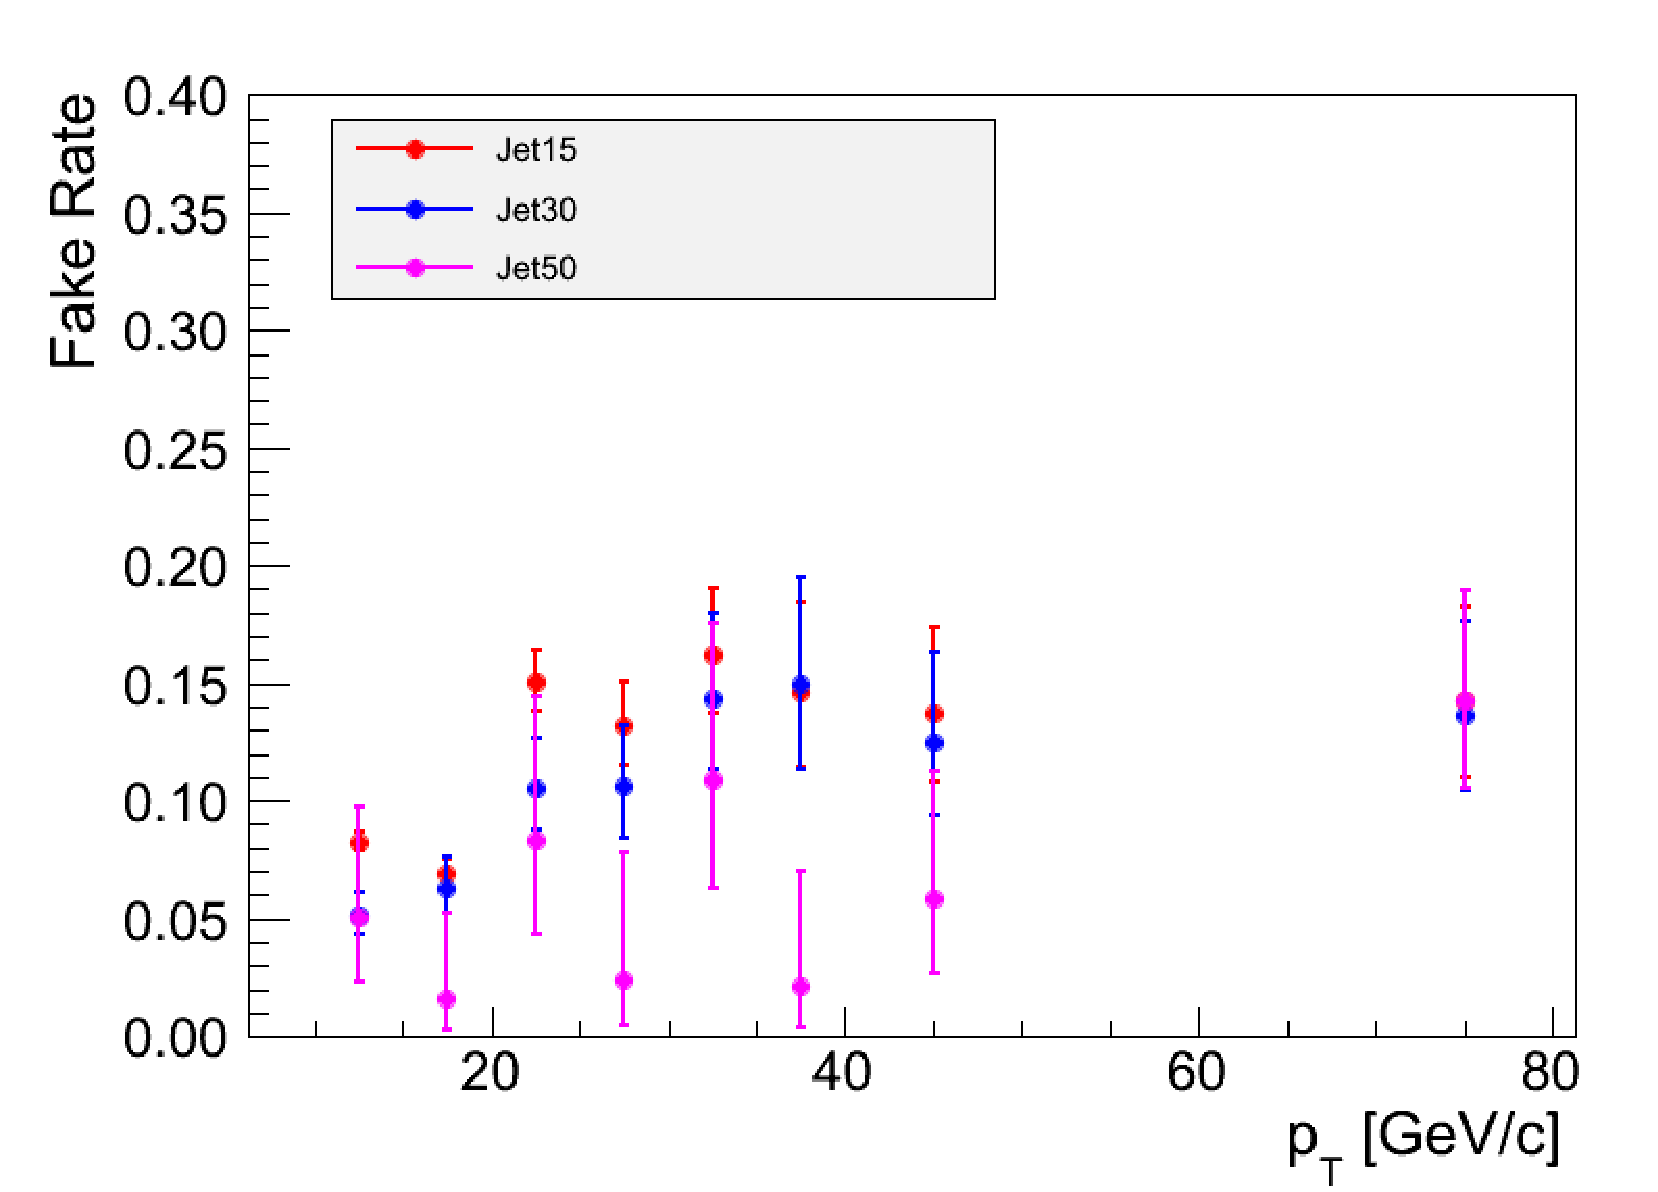
\includegraphics[width=0.45\textwidth]{figures/ElectronFakeRate_DenominatorV4_Ele8CaloIdLCaloIsoVLSample_Pt.pdf}}
\caption{Fake rates for the different fakeable object definitions, as a function of $p_T$, showing
the dependence on the $p_{T}$ threshold of the leading jet in the event.}
\label{fig:ele_fr_jetPtThresholdDependence}
\end{center}
\end{figure}

Due to the fact that the jet $p_{T}$ primarily affects the efficiency of the isolation cut,
we observe rather large differences between the different jet $p_{T}$ threshold samples
for the V1 and V3 fakeable object, where extrapolations in isolation are made. The V4 
denominator exhibits smaller systematic uncertainties since loose isolation cuts are 
already imposed on the denominator. The V2 fakeable object exhibits negligible 
systematic uncertainty since it is already fully isolated. 

These jet $p_{T}$ systematic uncertainties give a rough estimate of the uncertainty on the fake rate. 
We intend to improve the understanding of this aspect of the fake rate in the next iteration of the
analysis, by reweighting the jet $p_{T}$ in the fake rate measurement sample to the 
jet $p_{T}$ distribution in the W+Jet Monte Carlo
simulation. This procedure is expected to significantly decrease the jet $p_{T}$ systematic
uncertainty.



%% \subsubsection{Run dependence}

%% - fake rates can be affected by run and detector conditions.
%% - we demonstrate how much run dependence there is


 \subsubsection{Closure Test}
 To quantify the systematic uncertainties in extrapolating from the QCD dominated fake rate
calibration sample to the W+Jet dominated application sample, we perform a closure test using 
the Monte Carlo simulation. Fake rates measured from a cross-section weighted combination of 
the QCD Monte Carlo samples, generated with pt-hat $15-30$ GeV and $30-50$ GeV, are applied on
a W+Jet Monte Carlo sample. To measure the fake rate, the selection documented in Section
\ref{sec:ElectronFakeRate_CalibrationSampleSelection} is used as in data, with a $p_{T}$ 
threshold of $30$ GeV on the leading jet in the event. These predictions of yields and 
distributions are compared with the yields and distributions obtained from the 
simulation-based result after the WW selection. The sample is normalized to the 
total number of Monte Carlo events in the W+Jet sample, corresponding roughly to $3$ \ifb.
To ensure that we compare only the relevent components of the fake electron background,
we remove any events containing fake muons or W+$\gamma$ events with a generator level photon 
produced with $p_{T} > 10$ GeV. In the subsequent results, only the statistical uncertainty 
from the limited sample size is shown. The statistical uncertainty from the limited size of 
the fake rate measurement sample are not propagated. 

Figure \ref{fig:FakeElectronClosureTest_FakeElePt} shows the comparison of the $p_{T}$
distribution of the fake electron predicted by the fake rate method and the full simulation,
after the dilepton selection and the WW pre-selection. The difference that is observed 
reflects the systematic uncertainty of the fake rate extrapolation between the different
event samples. 

\begin{figure}[!htbp]
\begin{center}
\subfigure[After dilepton selection]{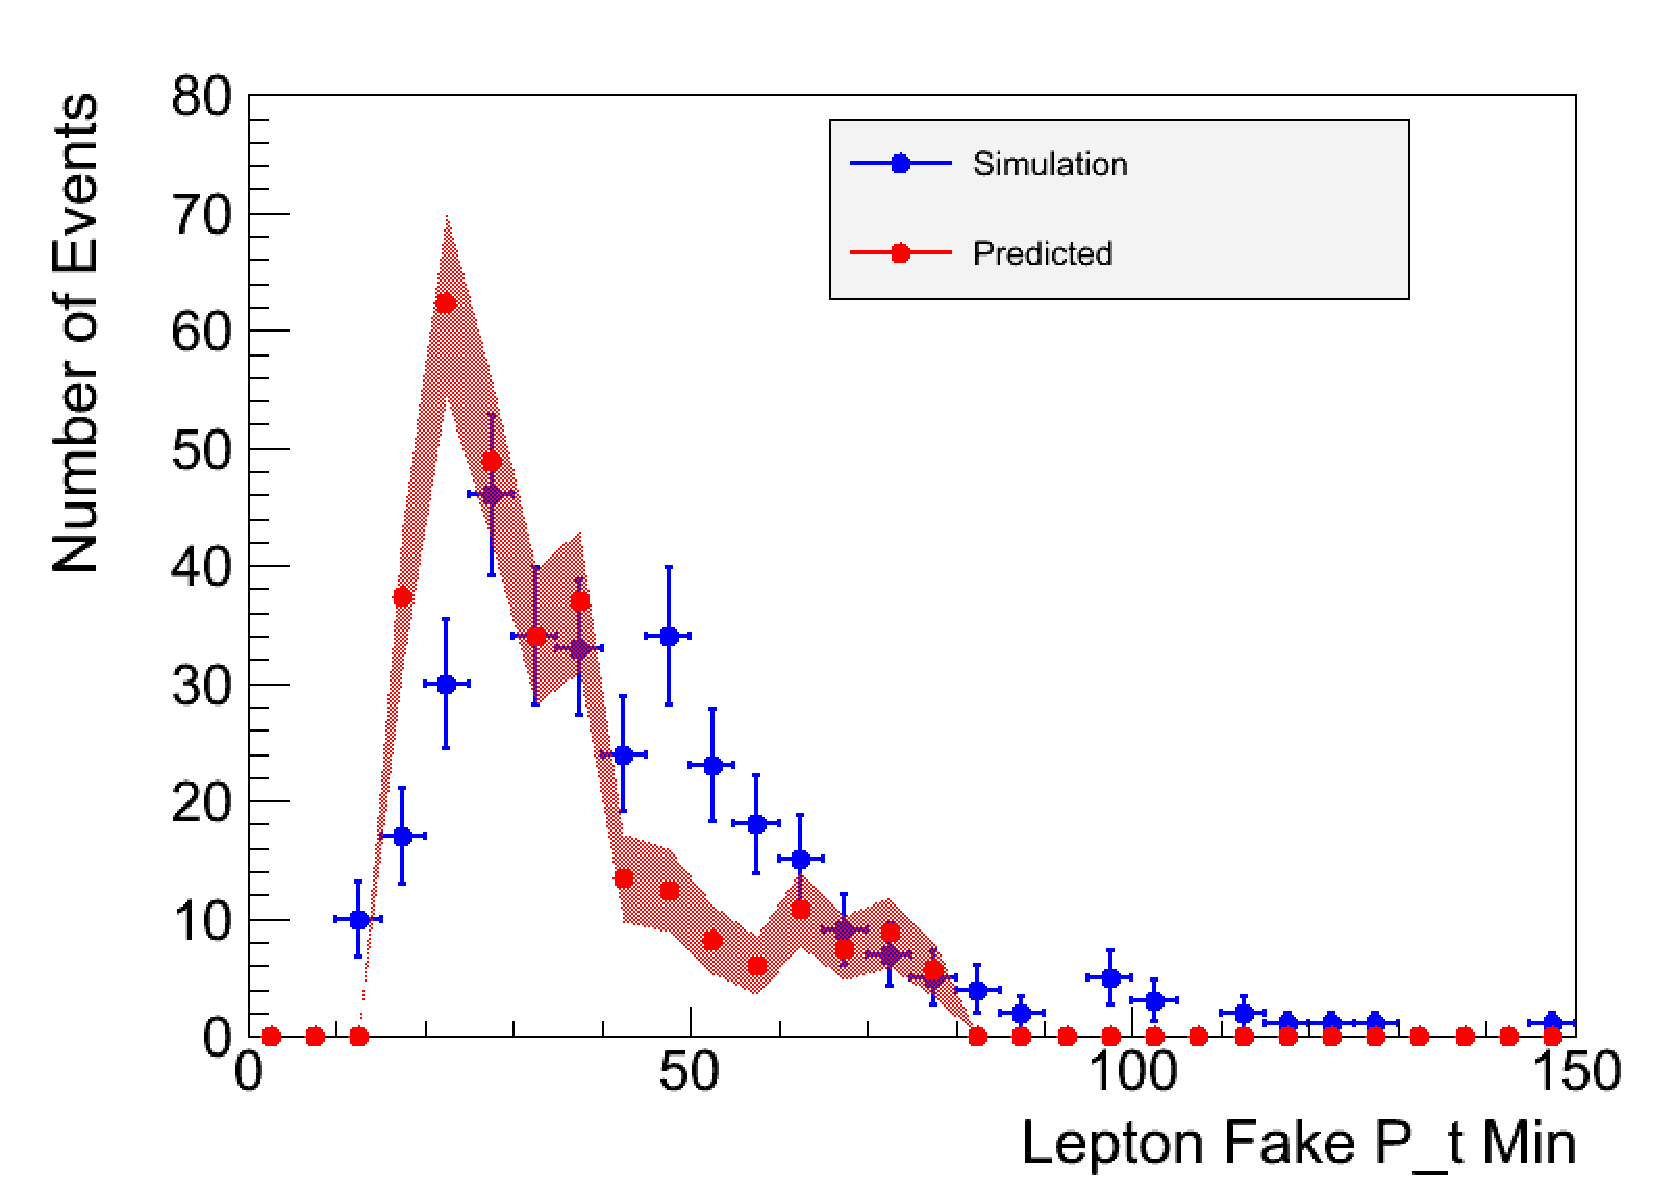
\includegraphics[width=0.45\textwidth]{figures/FakeElectronClosureTest_FakeElePt_PreSelection.pdf}}
\subfigure[After WW selection]{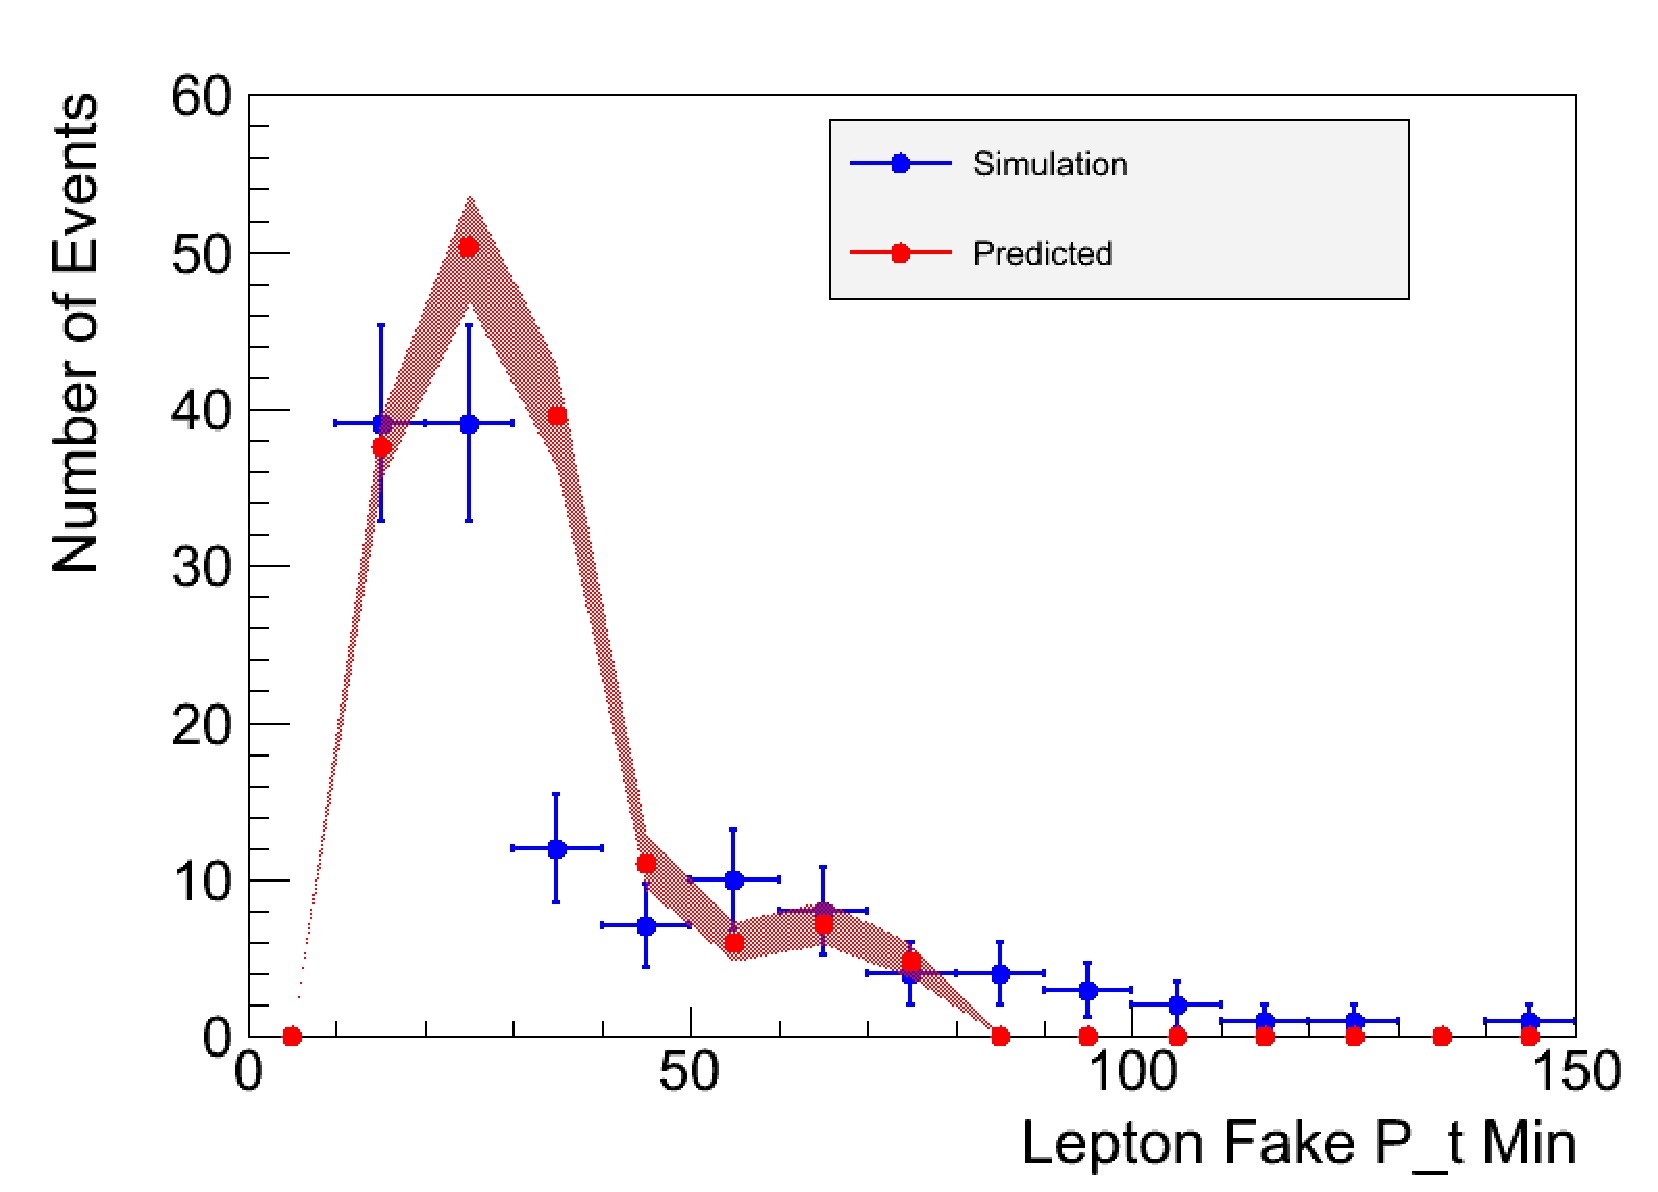
\includegraphics[width=0.45\textwidth]{figures/FakeElectronClosureTest_FakeElePt.pdf}}
\caption{The $p_{T}$ distribution for the fake electron, after dilepton selection and after
WW selection, is compared between the fake rate method prediction and the simulation prediction. }
\label{fig:FakeElectronClosureTest_FakeElePt}
\end{center}
\end{figure}

Table \ref{tab:FakeElectronClosureTest_Yields} summarizes the comparison between the
predicted yields and the yields from the Monte Carlo simulation, at various stages
of the Higgs selection. At all stages of the selection, the relative difference
between the predicted yield and the simulated yield is less than about $20\%$. 
At the final higgs selection level, the difference in the total yield is about
$30\%$, but suffers from statistical uncertainties due to the limited Monte Carlo 
sample size. 

\begin{table}[!htbp]
\begin{center}
\begin{tabular}{|l|c|c|c|}
\hline
\multicolumn{4}{|c|}{After dilepton selection} \\
\hline
Final State     & Predicted Yield   & Simulation Yield & Fractional Difference\\
\hline
ee              &  $193 \pm 10$     & $203 \pm 14$     & $-5\%$\\
e $\mu$         &  $250 \pm 11$     & $203 \pm 14$     & $+23\%$\\
total           &  $443 \pm 15$     & $406 \pm 20$     & $+9\%$\\
\hline
\multicolumn{4}{|c|}{After dilepton selection and $\met > 20$ GeV, $M_{\mathrm{ll}} > 12$ GeV cuts} \\
\hline
Final State     & Predicted Yield   & Simulation Yield & Fractional Difference\\
\hline
ee              &  $126 \pm 9$      & $164 \pm 13$     & $-23\%$\\
e $\mu$         &  $168 \pm 10$     & $169 \pm 13$     & $-1\%$\\
total           &  $295 \pm 13$     & $333 \pm 18$     & $-11\%$\\
\hline
\multicolumn{4}{|c|}{After WW selection} \\
\hline
Final State     & Predicted Yield   & Simulation Yield & Fractional Difference\\
\hline
ee              &  $36.2  \pm 4.9$  & $33  \pm  5.7$   & $+10\%$  \\
e $\mu$         &  $93.8  \pm 6.7$  & $105 \pm 10.2$   & $-11\%$  \\
total           &  $130.0 \pm 8.3$  & $138 \pm 11.7$   & $-6\%$  \\
\hline
\multicolumn{4}{|c|}{After HWW 130 selection} \\
\hline
Final State     & Predicted Yield   & Simulation Yield & Fractional Difference\\
\hline
ee              &  $3.2  \pm 0.9$   & $8  \pm 2.8$     & $-60\%$\\
e $\mu$         &  $9.8  \pm 1.7$   & $11 \pm 3.3$     & $-11\%$\\
total           &  $13.1 \pm 2.0$   & $19 \pm 4.4$     & $-31\%$\\
\hline
\end{tabular}
\caption{Comparison of fake electron background yields at various stages of the 
analysis selection between the fake rate method prediction and the simulation
prediction. }
\label{tab:FakeElectronClosureTest_Yields}
\end{center}
\end{table}

Figure \ref{fig:FakeElectronClosureTest_LeptonPt} shows the comparison of the $p_{T}$
of the leading and trailing leptons after the WW selection between the prediction
from the fake rate method and from the simulation. Analogous comparisons for 
the missing transverse energy, the dilepton mass, and the $\Delta\phi$ between 
the two leptons are shown in Figure \ref{fig:FakeElectronClosureTest_MoreObservables}.
There are no major systematic differences observed in any of these distributions 
beyond the $20-30\%$ level. Finally, Figure \ref{fig:FakeElectronClosureTest_CutFlow}
shows the comparison of the cut flow for the $ee$ and $e\mu$ final states between
the prediction from the fake rate method and the simulation. Again, no major 
discrepancies beyond the $20-30\%$ level are observed. 


\begin{figure}[!htbp]
\begin{center}
\subfigure[Leading lepton $p_{T}$]{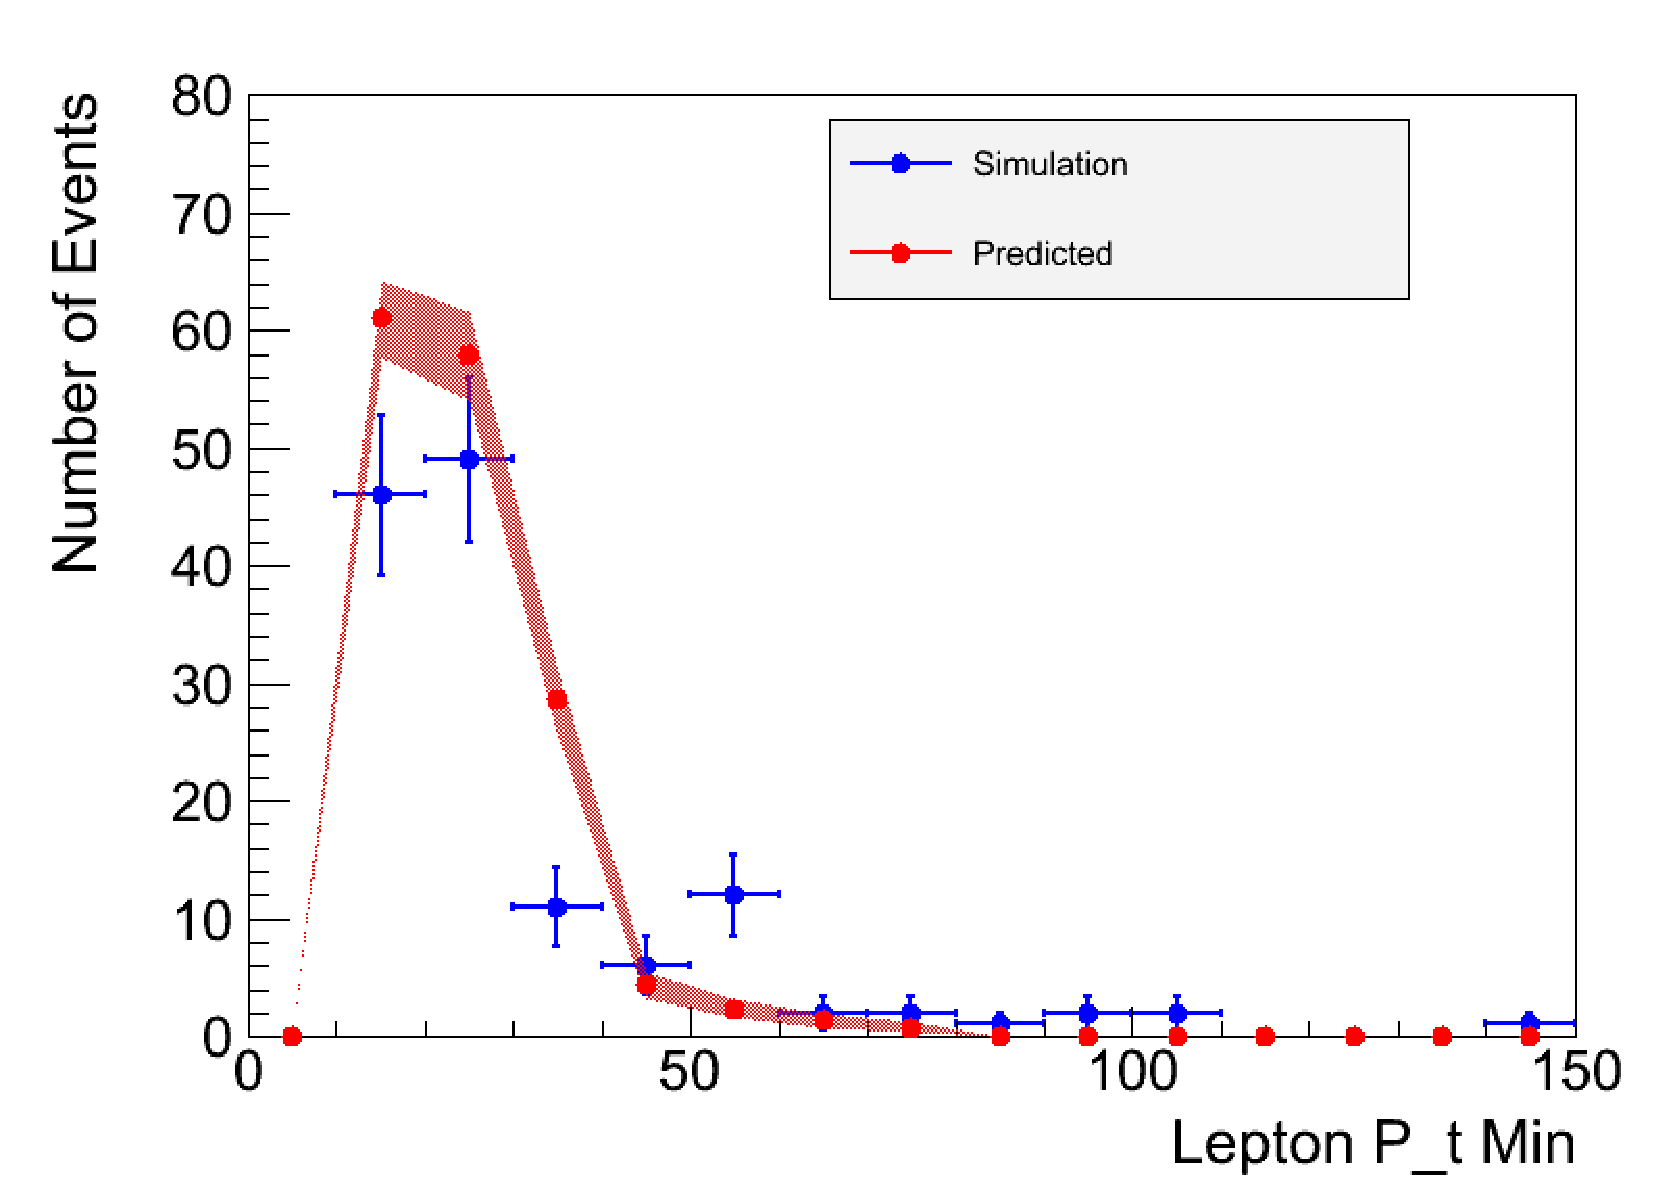
\includegraphics[width=0.45\textwidth]{figures/FakeElectronClosureTest_PtMin.pdf}}
\subfigure[Trailing lepton $p_{T}$]{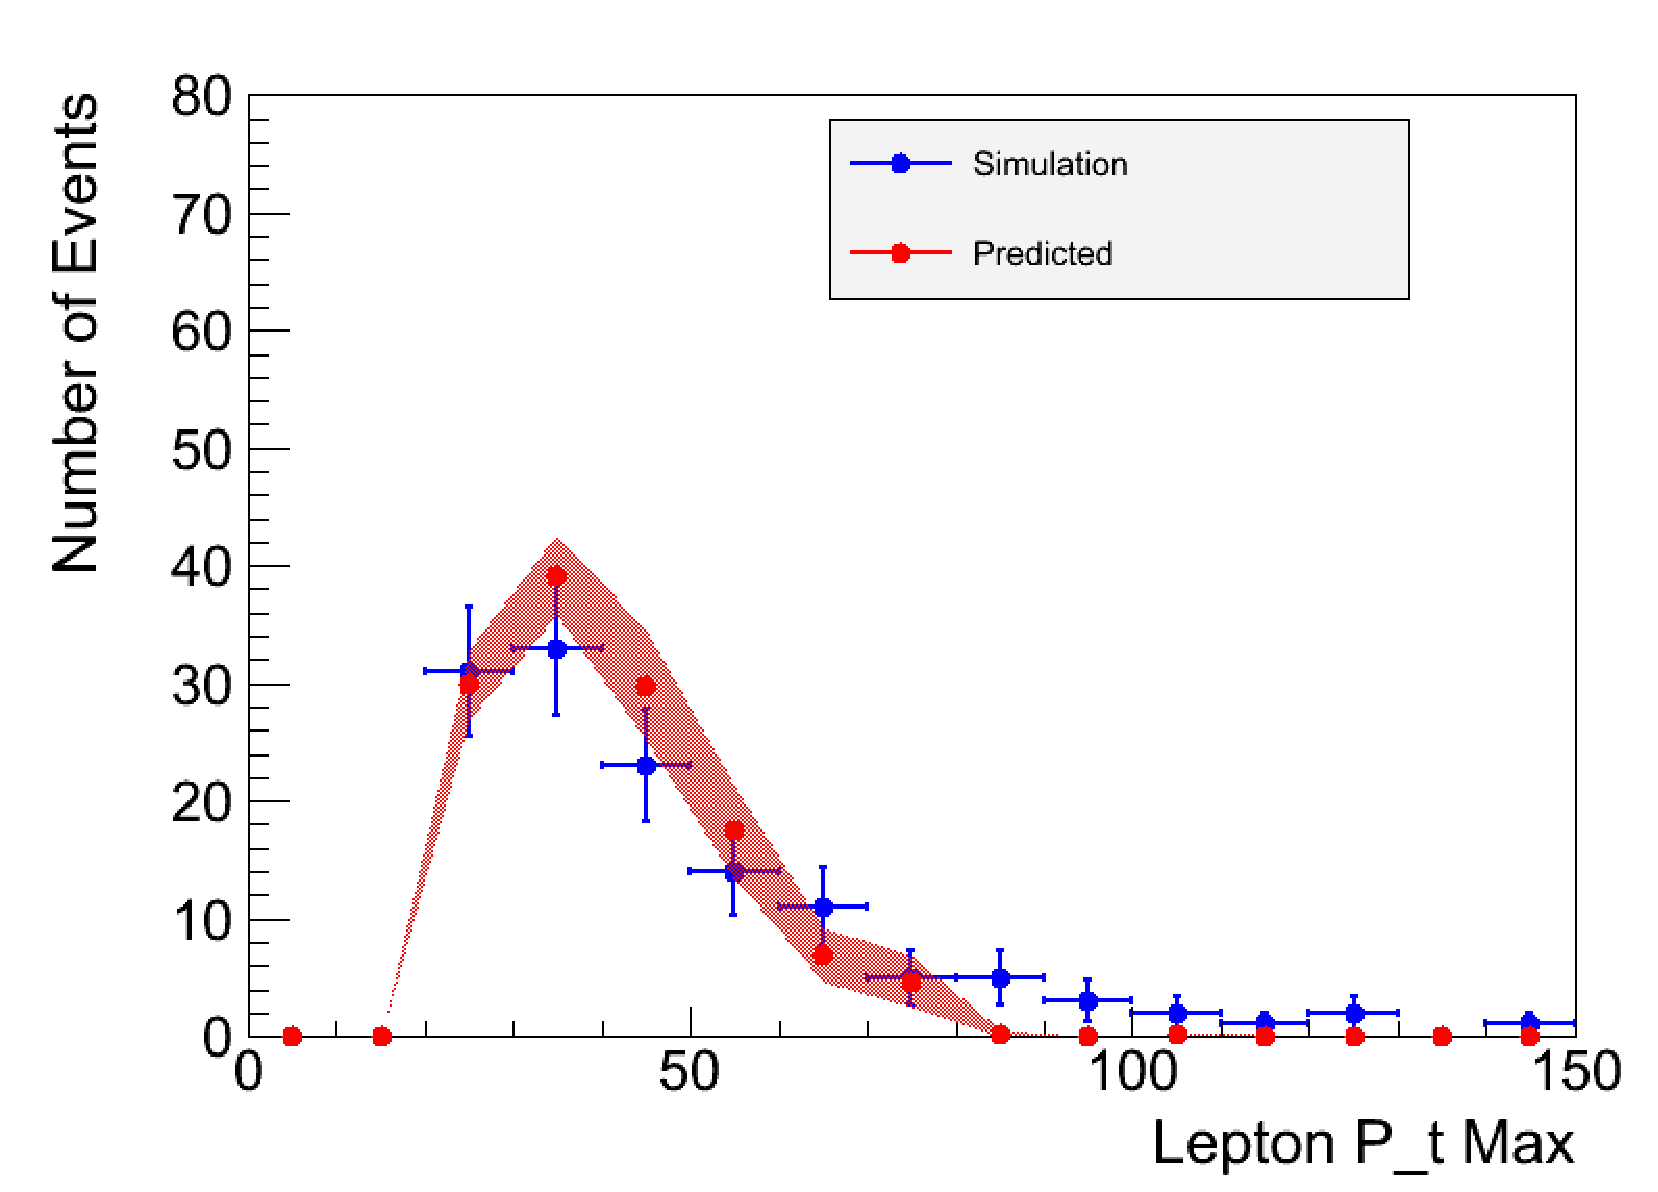
\includegraphics[width=0.45\textwidth]{figures/FakeElectronClosureTest_PtMax.pdf}}
\caption{A comparison of the $p_{T}$ distribution of the leading and trailing lepton
between the fake rate method prediction and the simulation prediction. }
\label{fig:FakeElectronClosureTest_LeptonPt}
\end{center}
\end{figure}

\begin{figure}[!htbp]
\begin{center}
\subfigure[$\met$]{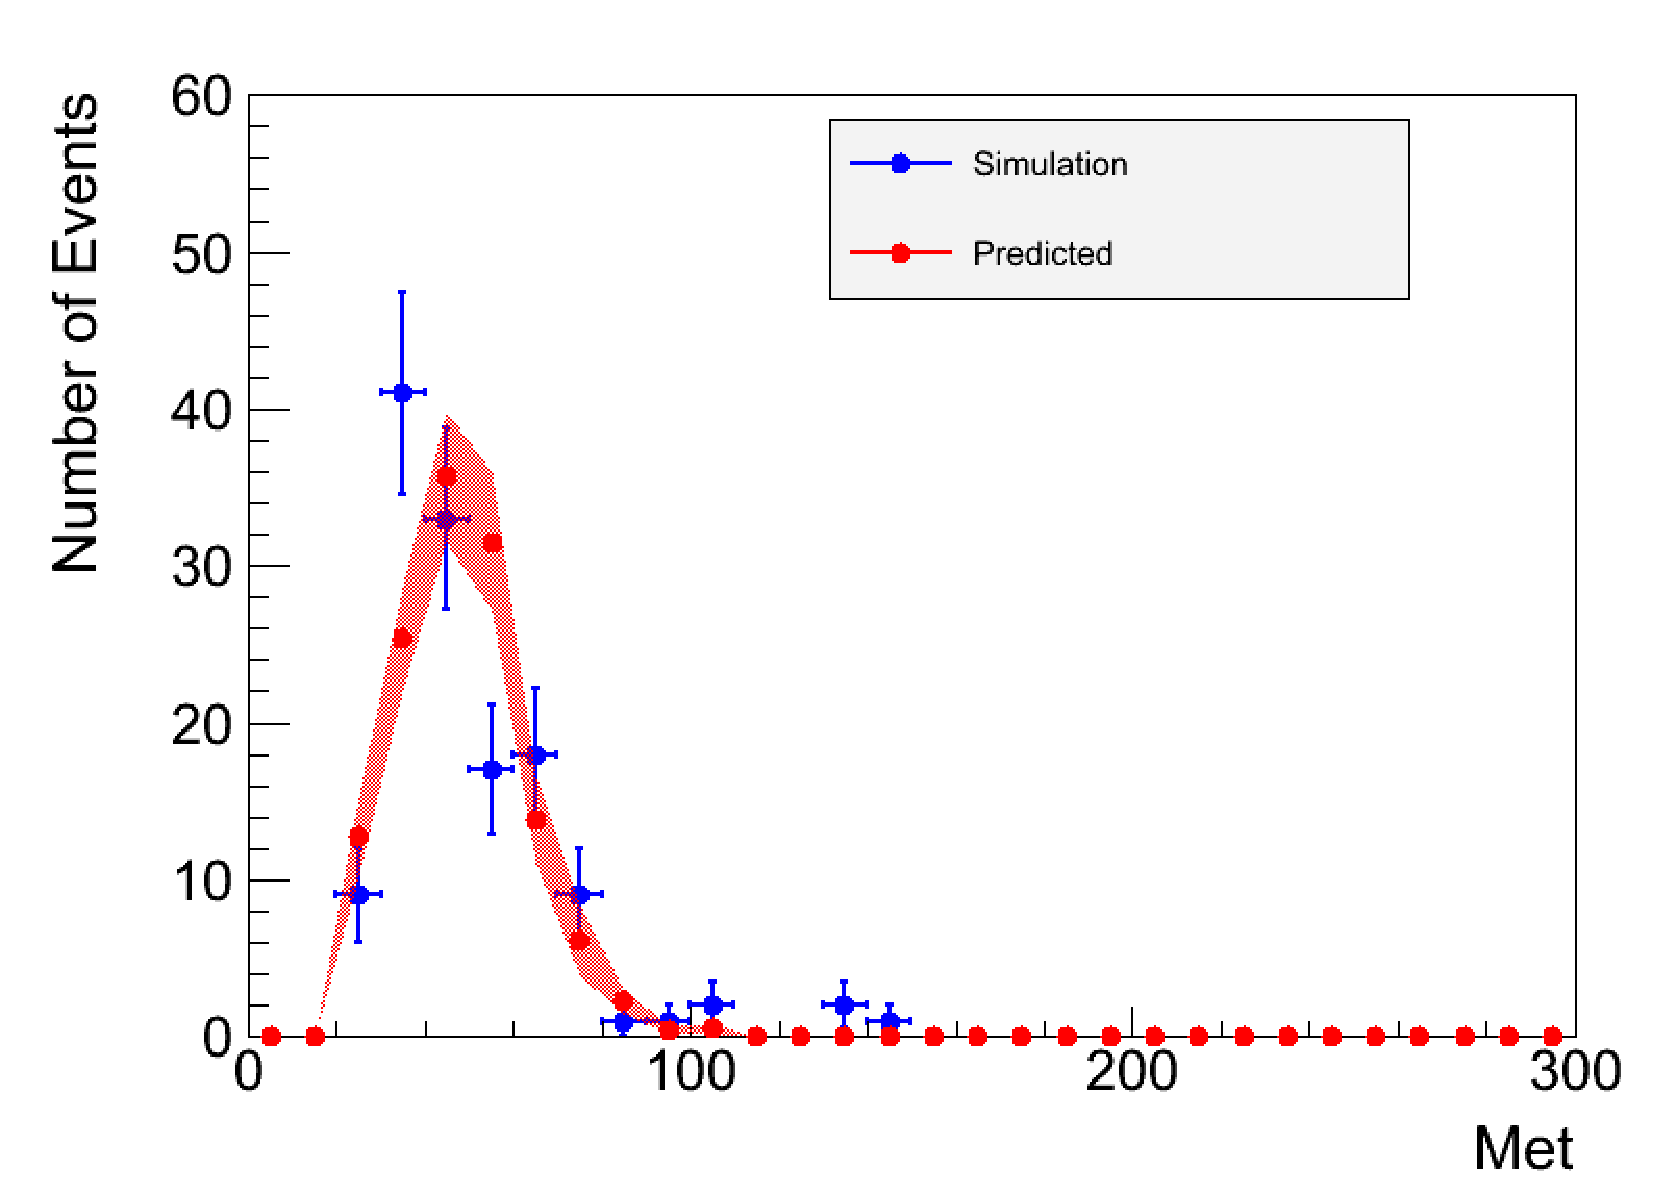
\includegraphics[width=0.45\textwidth]{figures/FakeElectronClosureTest_Met.pdf}}
\subfigure[Dilepton Mass]{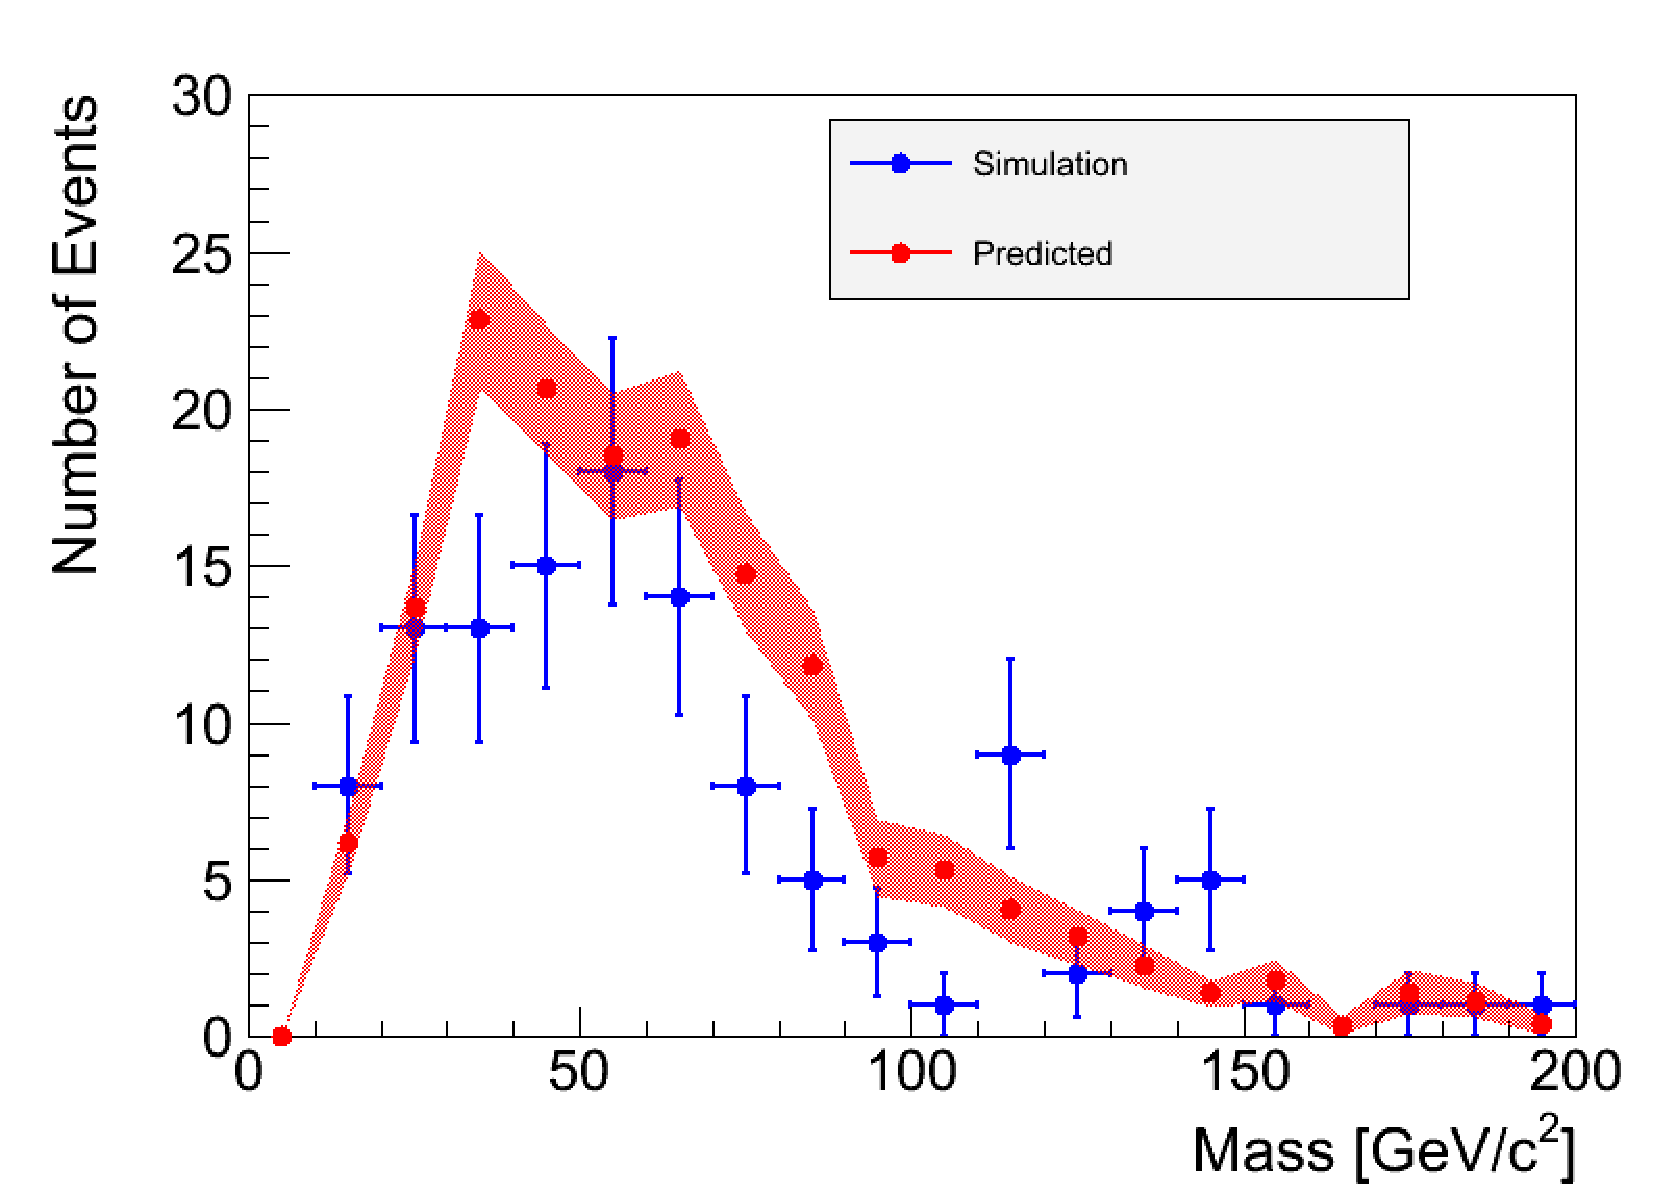
\includegraphics[width=0.45\textwidth]{figures/FakeElectronClosureTest_DileptonMass.pdf}}
\subfigure[$\Delta\phi$]{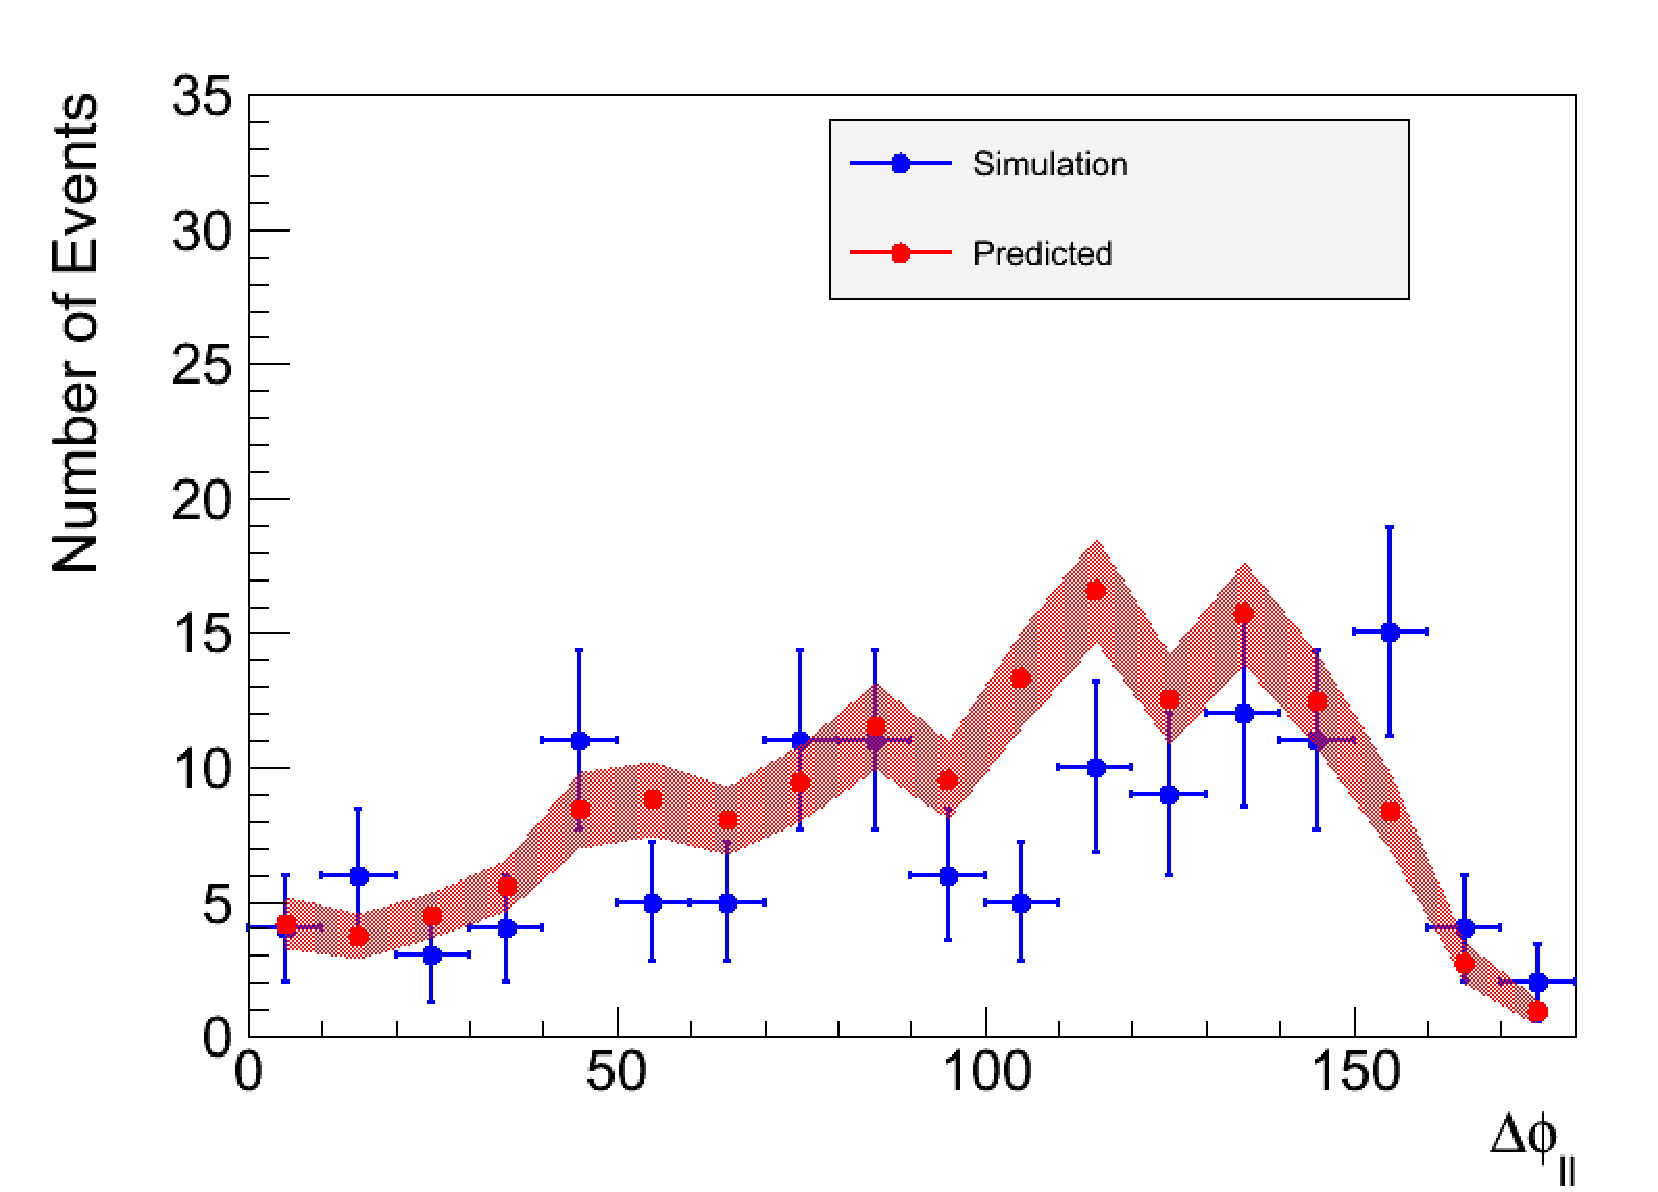
\includegraphics[width=0.45\textwidth]{figures/FakeElectronClosureTest_DeltaPhi.pdf}}
\caption{A comparison of the distribution of the missing transverse energy, the dilepton mass, 
and the $\Delta\phi$ between the two leptons predicted using the fake rate method and the
full simulation.}
\label{fig:FakeElectronClosureTest_MoreObservables}
\end{center}
\end{figure}

\begin{figure}[!htbp]
\begin{center}
\subfigure[ee]{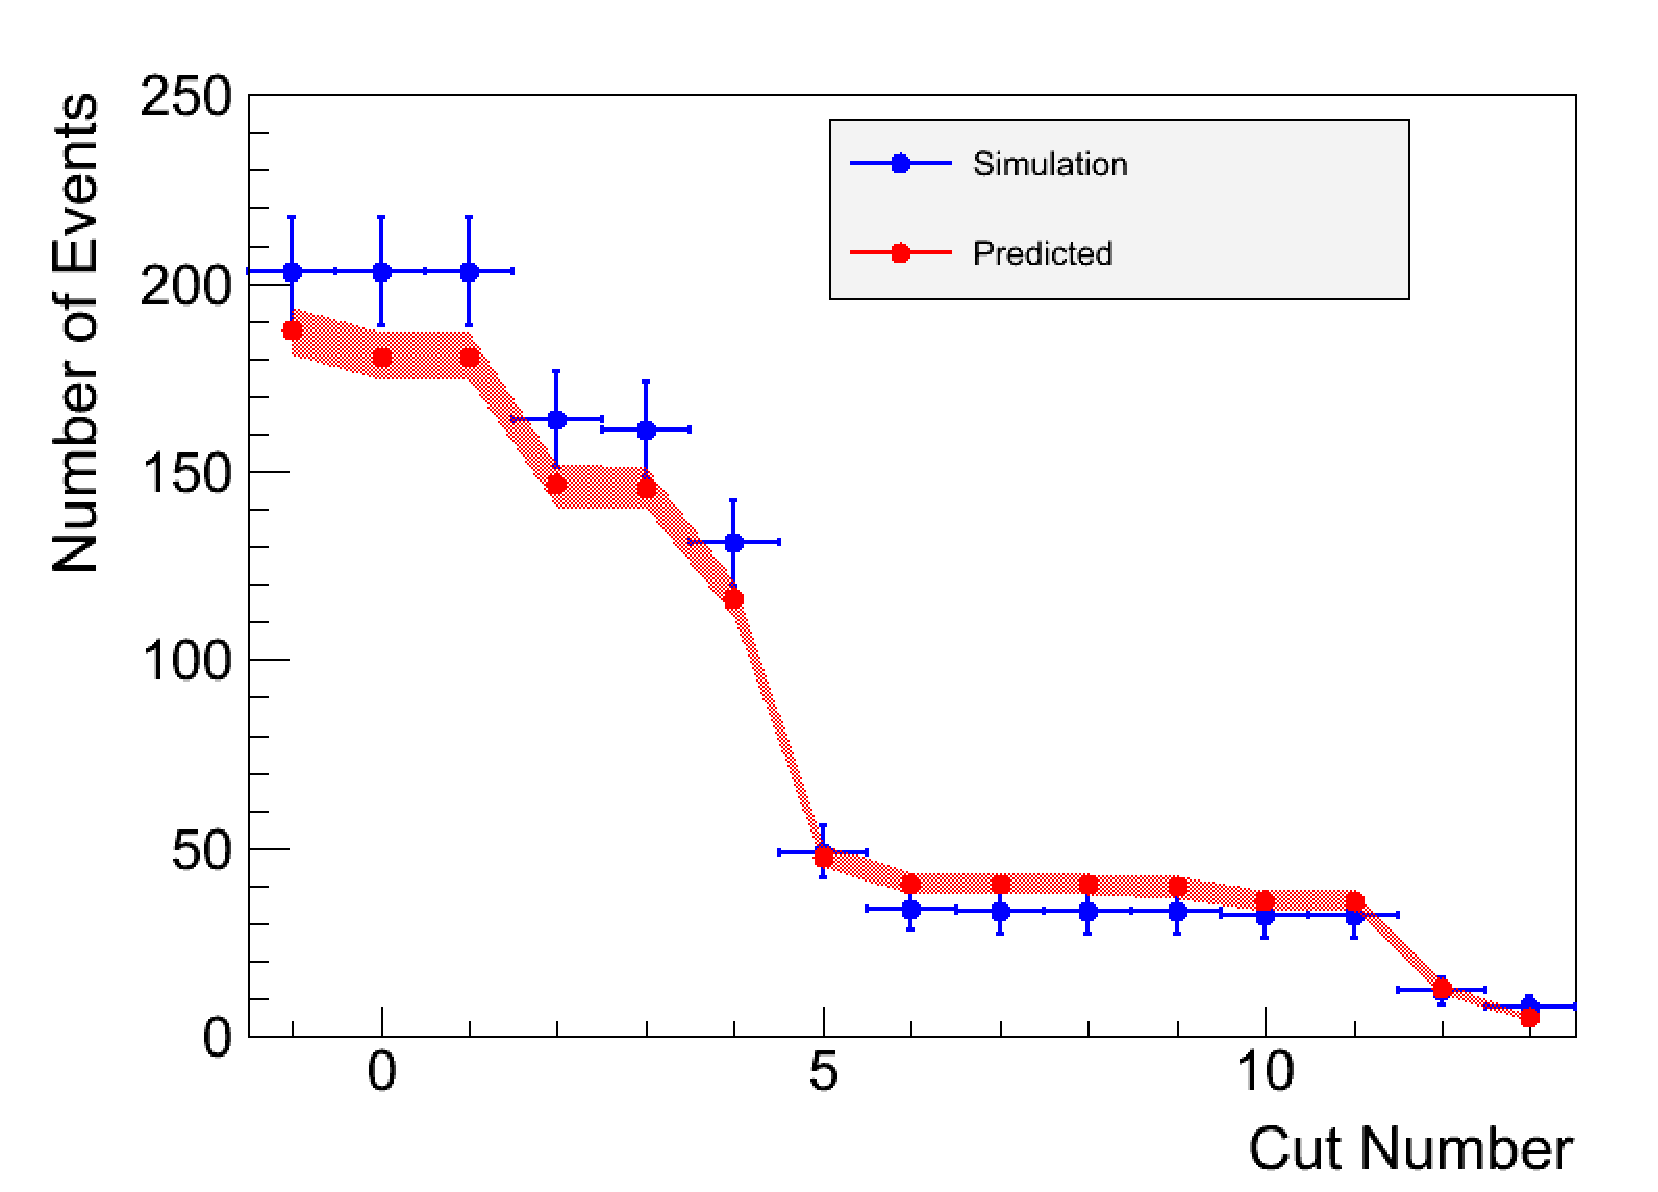
\includegraphics[width=0.45\textwidth]{figures/FakeElectronClosureTest_CutFlowEE.pdf}}
\subfigure[e$\mu$]{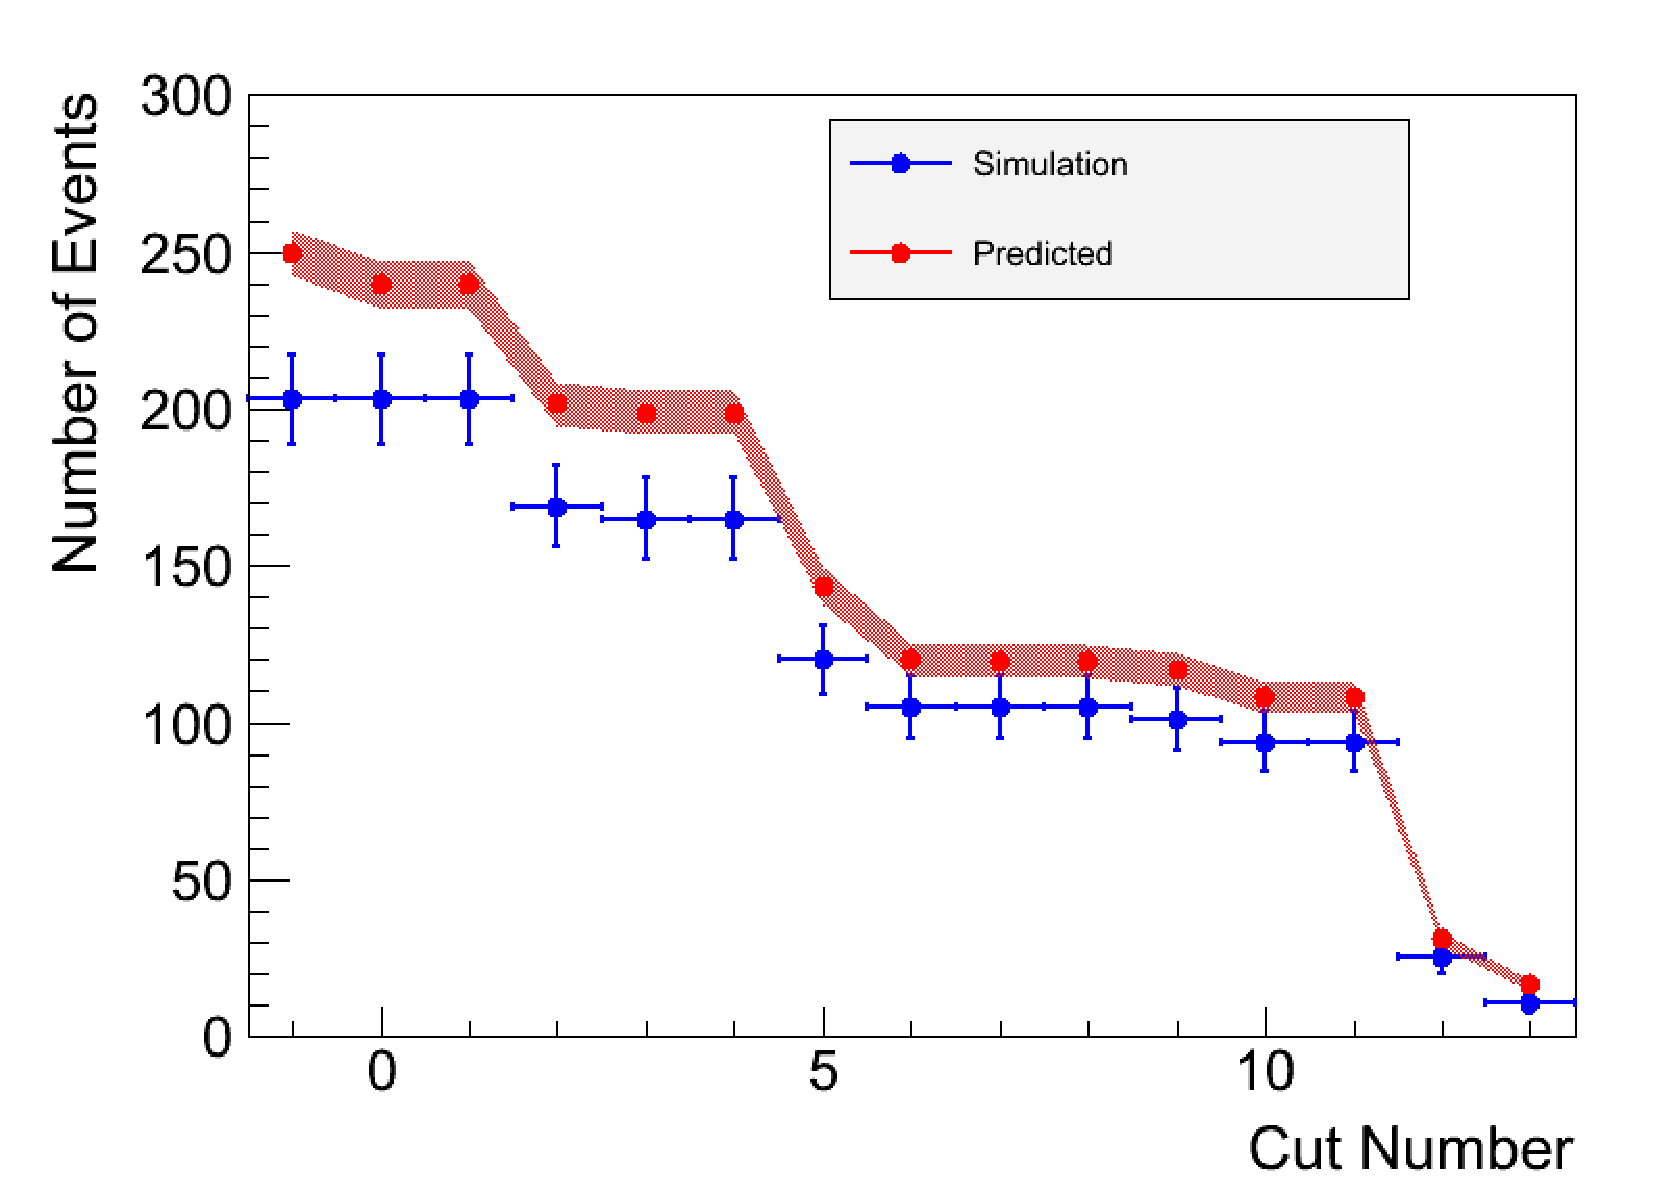
\includegraphics[width=0.45\textwidth]{figures/FakeElectronClosureTest_CutFlowEMu.pdf}}
\caption{A comparison of the cut flow of the W+Jet background for the ee and e$\mu$ final states
between the fake rate method prediction and the full simulation prediction. }
\label{fig:FakeElectronClosureTest_CutFlow}
\end{center}
\end{figure}

To summarize, ignoring the yield comparison after the final Higgs selection cuts which 
suffer from large statistical uncertainties, we estimate a systematic uncertainty of 
$25\%$ for the fake electron background prediction due to the sample extrapolation 
coming from the largest differences observed in the yields of the closure test from 
Table \ref{tab:FakeElectronClosureTest_Yields}. 

%% \subsubsection{Data prediction}

%% - describe how we propagate uncertainties
%%   - assume statistical uncertainties are uncorrelated per bin
%%   - assume systematics are 100\% correlated
